\documentclass[aspectratio=169]{beamer}
% Shared preamble for ml/ slide decks.
% Each lecture .tex starts with:
%   \documentclass[aspectratio=169]{beamer}
%   % Shared preamble for ml/ slide decks.
% Each lecture .tex starts with:
%   \documentclass[aspectratio=169]{beamer}
%   % Shared preamble for ml/ slide decks.
% Each lecture .tex starts with:
%   \documentclass[aspectratio=169]{beamer}
%   \input{../preamble}
% Compile from inside the chapter folder so \input{../preamble} resolves.

\usetheme{default}
\usecolortheme{dove}

\setbeamertemplate{navigation symbols}{}
\setbeamertemplate{footline}{%
  \hfill{\large\insertframenumber\,/\,\inserttotalframenumber}\hspace{0.8em}\vspace{0.5em}%
}

% Project palette (existing, kept for backwards compatibility with deferred/*)
\definecolor{popblue}{RGB}{52, 101, 164}
\definecolor{sampred}{RGB}{204, 0, 0}
\definecolor{paramgreen}{RGB}{0, 140, 70}
\definecolor{warnred}{RGB}{180, 40, 40}
\definecolor{orange1}{RGB}{220, 120, 0}
\definecolor{violet1}{RGB}{120, 50, 160}
\definecolor{lightbg}{RGB}{245, 245, 250}

% Armenian flag palette (use these for any 3-color highlight; per CLAUDE.md).
% "Nice versions": slightly de-saturated from the official spec for slide use,
% so they don't burn out under projector colors. Originals kept as *_pure.
\definecolor{armred}{RGB}{200, 30, 40}      % nice red (official #D90012 muted)
\definecolor{armblue}{RGB}{30, 70, 160}     % nice blue (official #0033A0 muted)
\definecolor{armorange}{RGB}{230, 160, 30}  % nice orange (official #F2A800 muted)
\definecolor{armred_pure}{HTML}{D90012}     % official Armenian flag red
\definecolor{armblue_pure}{HTML}{0033A0}    % official Armenian flag blue
\definecolor{armorange_pure}{HTML}{F2A800}  % official Armenian flag orange

\setbeamercolor{frametitle}{fg=popblue}
\setbeamercolor{title}{fg=popblue}

\usepackage{pgfplots}
\usepackage{tikz}
\usetikzlibrary{shapes, arrows.meta, positioning, calc, decorations.pathreplacing, patterns, matrix}
\pgfplotsset{compat=1.18}
\usepackage{amsmath, amssymb, amsfonts}
\usepackage{bm}
\usepackage{dsfont}
\usepackage{array}
\usepackage{pifont}
\usepackage{colortbl}
\usepackage{fontenc}

% Callout boxes. Purely additive - existing decks are unaffected.
% Usage: \begin{tcolorbox}[colback=armblue!8, colframe=armblue, boxrule=0.6pt, arc=2pt,
%                          title=\textbf{Key idea}] ... \end{tcolorbox}
% Palette convention (ml/SLIDE_STYLE.md): armblue=key idea, armred=trap/warning,
% paramgreen=takeaway or "Next", armorange=watch-out.
\usepackage[most]{tcolorbox}

% Cleaner table rules (\toprule, \midrule, \bottomrule). Also purely additive.
\usepackage{booktabs}

% \cancel{...} for struck-through terms in derivations (added 2026-08-11 for the
% importance-sampling frame in ch11_rl, where the dynamics cancel). Purely additive.
\usepackage{cancel}

% Minimal ML notation macros (subset of slds-lmu latex-math/basic-ml.tex).
% Kept here so we don't have to inline-expand every \thetav, \xv, etc.
% when porting upstream slides.
\newcommand{\R}{\mathds{R}}
\newcommand{\N}{\mathds{N}}
\newcommand{\E}{\mathds{E}}
\newcommand{\Xspace}{\mathcal{X}}
\newcommand{\Yspace}{\mathcal{Y}}
\newcommand{\Hspace}{\mathcal{H}}
\newcommand{\D}{\mathcal{D}}
\newcommand{\Dtrain}{\mathcal{D}_{\text{train}}}
\newcommand{\Dtest}{\mathcal{D}_{\text{test}}}
\newcommand{\xv}{\mathbf{x}}
\newcommand{\yv}{\mathbf{y}}
\newcommand{\Xmat}{\mathbf{X}}
\newcommand{\id}{\mathbf{I}}
\newcommand{\thetav}{\bm{\theta}}
\newcommand{\thetah}{\hat{\bm{\theta}}}
\newcommand{\lamv}{\bm{\lambda}}
\newcommand{\fx}{f(\xv)}
\newcommand{\fxt}{f(\xv \,|\, \bm{\theta})}
\newcommand{\fxi}{f\!\left(\xv^{(i)}\right)}
\newcommand{\fh}{\hat{f}}
\newcommand{\fxh}{\hat{f}(\xv)}
\newcommand{\yh}{\hat{y}}
\newcommand{\yih}{\hat{y}^{(i)}}
% \xi clashes with the Greek letter \xi; write \xv^{(i)} inline instead.
\newcommand{\yi}[1][i]{y^{(#1)}}
\newcommand{\xyi}[1][i]{\left(\xv^{(#1)},\, y^{(#1)}\right)}
\newcommand{\thx}{\bm{\theta}^\top \xv}
\newcommand{\sumin}{\sum_{i=1}^{n}}
\newcommand{\sumjp}{\sum_{j=1}^{p}}
\newcommand{\Lxy}{L\!\left(y, \fx\right)}
\newcommand{\Lxyi}{L\!\left(\yi, \fxi\right)}
\newcommand{\risk}{\mathcal{R}}
\newcommand{\riske}{\mathcal{R}_{\text{emp}}}
\newcommand{\risket}{\mathcal{R}_{\text{emp}}(\bm{\theta})}
\newcommand{\riskt}{\mathcal{R}(\bm{\theta})}
\newcommand{\riskr}{\mathcal{R}_{\text{reg}}}
\newcommand{\argmin}{\mathop{\mathrm{arg\,min}}}
\newcommand{\argmax}{\mathop{\mathrm{arg\,max}}}
\newcommand{\eps}{\varepsilon}

% Compile from inside the chapter folder so % Shared preamble for ml/ slide decks.
% Each lecture .tex starts with:
%   \documentclass[aspectratio=169]{beamer}
%   \input{../preamble}
% Compile from inside the chapter folder so \input{../preamble} resolves.

\usetheme{default}
\usecolortheme{dove}

\setbeamertemplate{navigation symbols}{}
\setbeamertemplate{footline}{%
  \hfill{\large\insertframenumber\,/\,\inserttotalframenumber}\hspace{0.8em}\vspace{0.5em}%
}

% Project palette (existing, kept for backwards compatibility with deferred/*)
\definecolor{popblue}{RGB}{52, 101, 164}
\definecolor{sampred}{RGB}{204, 0, 0}
\definecolor{paramgreen}{RGB}{0, 140, 70}
\definecolor{warnred}{RGB}{180, 40, 40}
\definecolor{orange1}{RGB}{220, 120, 0}
\definecolor{violet1}{RGB}{120, 50, 160}
\definecolor{lightbg}{RGB}{245, 245, 250}

% Armenian flag palette (use these for any 3-color highlight; per CLAUDE.md).
% "Nice versions": slightly de-saturated from the official spec for slide use,
% so they don't burn out under projector colors. Originals kept as *_pure.
\definecolor{armred}{RGB}{200, 30, 40}      % nice red (official #D90012 muted)
\definecolor{armblue}{RGB}{30, 70, 160}     % nice blue (official #0033A0 muted)
\definecolor{armorange}{RGB}{230, 160, 30}  % nice orange (official #F2A800 muted)
\definecolor{armred_pure}{HTML}{D90012}     % official Armenian flag red
\definecolor{armblue_pure}{HTML}{0033A0}    % official Armenian flag blue
\definecolor{armorange_pure}{HTML}{F2A800}  % official Armenian flag orange

\setbeamercolor{frametitle}{fg=popblue}
\setbeamercolor{title}{fg=popblue}

\usepackage{pgfplots}
\usepackage{tikz}
\usetikzlibrary{shapes, arrows.meta, positioning, calc, decorations.pathreplacing, patterns, matrix}
\pgfplotsset{compat=1.18}
\usepackage{amsmath, amssymb, amsfonts}
\usepackage{bm}
\usepackage{dsfont}
\usepackage{array}
\usepackage{pifont}
\usepackage{colortbl}
\usepackage{fontenc}

% Callout boxes. Purely additive - existing decks are unaffected.
% Usage: \begin{tcolorbox}[colback=armblue!8, colframe=armblue, boxrule=0.6pt, arc=2pt,
%                          title=\textbf{Key idea}] ... \end{tcolorbox}
% Palette convention (ml/SLIDE_STYLE.md): armblue=key idea, armred=trap/warning,
% paramgreen=takeaway or "Next", armorange=watch-out.
\usepackage[most]{tcolorbox}

% Cleaner table rules (\toprule, \midrule, \bottomrule). Also purely additive.
\usepackage{booktabs}

% \cancel{...} for struck-through terms in derivations (added 2026-08-11 for the
% importance-sampling frame in ch11_rl, where the dynamics cancel). Purely additive.
\usepackage{cancel}

% Minimal ML notation macros (subset of slds-lmu latex-math/basic-ml.tex).
% Kept here so we don't have to inline-expand every \thetav, \xv, etc.
% when porting upstream slides.
\newcommand{\R}{\mathds{R}}
\newcommand{\N}{\mathds{N}}
\newcommand{\E}{\mathds{E}}
\newcommand{\Xspace}{\mathcal{X}}
\newcommand{\Yspace}{\mathcal{Y}}
\newcommand{\Hspace}{\mathcal{H}}
\newcommand{\D}{\mathcal{D}}
\newcommand{\Dtrain}{\mathcal{D}_{\text{train}}}
\newcommand{\Dtest}{\mathcal{D}_{\text{test}}}
\newcommand{\xv}{\mathbf{x}}
\newcommand{\yv}{\mathbf{y}}
\newcommand{\Xmat}{\mathbf{X}}
\newcommand{\id}{\mathbf{I}}
\newcommand{\thetav}{\bm{\theta}}
\newcommand{\thetah}{\hat{\bm{\theta}}}
\newcommand{\lamv}{\bm{\lambda}}
\newcommand{\fx}{f(\xv)}
\newcommand{\fxt}{f(\xv \,|\, \bm{\theta})}
\newcommand{\fxi}{f\!\left(\xv^{(i)}\right)}
\newcommand{\fh}{\hat{f}}
\newcommand{\fxh}{\hat{f}(\xv)}
\newcommand{\yh}{\hat{y}}
\newcommand{\yih}{\hat{y}^{(i)}}
% \xi clashes with the Greek letter \xi; write \xv^{(i)} inline instead.
\newcommand{\yi}[1][i]{y^{(#1)}}
\newcommand{\xyi}[1][i]{\left(\xv^{(#1)},\, y^{(#1)}\right)}
\newcommand{\thx}{\bm{\theta}^\top \xv}
\newcommand{\sumin}{\sum_{i=1}^{n}}
\newcommand{\sumjp}{\sum_{j=1}^{p}}
\newcommand{\Lxy}{L\!\left(y, \fx\right)}
\newcommand{\Lxyi}{L\!\left(\yi, \fxi\right)}
\newcommand{\risk}{\mathcal{R}}
\newcommand{\riske}{\mathcal{R}_{\text{emp}}}
\newcommand{\risket}{\mathcal{R}_{\text{emp}}(\bm{\theta})}
\newcommand{\riskt}{\mathcal{R}(\bm{\theta})}
\newcommand{\riskr}{\mathcal{R}_{\text{reg}}}
\newcommand{\argmin}{\mathop{\mathrm{arg\,min}}}
\newcommand{\argmax}{\mathop{\mathrm{arg\,max}}}
\newcommand{\eps}{\varepsilon}
 resolves.

\usetheme{default}
\usecolortheme{dove}

\setbeamertemplate{navigation symbols}{}
\setbeamertemplate{footline}{%
  \hfill{\large\insertframenumber\,/\,\inserttotalframenumber}\hspace{0.8em}\vspace{0.5em}%
}

% Project palette (existing, kept for backwards compatibility with deferred/*)
\definecolor{popblue}{RGB}{52, 101, 164}
\definecolor{sampred}{RGB}{204, 0, 0}
\definecolor{paramgreen}{RGB}{0, 140, 70}
\definecolor{warnred}{RGB}{180, 40, 40}
\definecolor{orange1}{RGB}{220, 120, 0}
\definecolor{violet1}{RGB}{120, 50, 160}
\definecolor{lightbg}{RGB}{245, 245, 250}

% Armenian flag palette (use these for any 3-color highlight; per CLAUDE.md).
% "Nice versions": slightly de-saturated from the official spec for slide use,
% so they don't burn out under projector colors. Originals kept as *_pure.
\definecolor{armred}{RGB}{200, 30, 40}      % nice red (official #D90012 muted)
\definecolor{armblue}{RGB}{30, 70, 160}     % nice blue (official #0033A0 muted)
\definecolor{armorange}{RGB}{230, 160, 30}  % nice orange (official #F2A800 muted)
\definecolor{armred_pure}{HTML}{D90012}     % official Armenian flag red
\definecolor{armblue_pure}{HTML}{0033A0}    % official Armenian flag blue
\definecolor{armorange_pure}{HTML}{F2A800}  % official Armenian flag orange

\setbeamercolor{frametitle}{fg=popblue}
\setbeamercolor{title}{fg=popblue}

\usepackage{pgfplots}
\usepackage{tikz}
\usetikzlibrary{shapes, arrows.meta, positioning, calc, decorations.pathreplacing, patterns, matrix}
\pgfplotsset{compat=1.18}
\usepackage{amsmath, amssymb, amsfonts}
\usepackage{bm}
\usepackage{dsfont}
\usepackage{array}
\usepackage{pifont}
\usepackage{colortbl}
\usepackage{fontenc}

% Callout boxes. Purely additive - existing decks are unaffected.
% Usage: \begin{tcolorbox}[colback=armblue!8, colframe=armblue, boxrule=0.6pt, arc=2pt,
%                          title=\textbf{Key idea}] ... \end{tcolorbox}
% Palette convention (ml/SLIDE_STYLE.md): armblue=key idea, armred=trap/warning,
% paramgreen=takeaway or "Next", armorange=watch-out.
\usepackage[most]{tcolorbox}

% Cleaner table rules (\toprule, \midrule, \bottomrule). Also purely additive.
\usepackage{booktabs}

% \cancel{...} for struck-through terms in derivations (added 2026-08-11 for the
% importance-sampling frame in ch11_rl, where the dynamics cancel). Purely additive.
\usepackage{cancel}

% Minimal ML notation macros (subset of slds-lmu latex-math/basic-ml.tex).
% Kept here so we don't have to inline-expand every \thetav, \xv, etc.
% when porting upstream slides.
\newcommand{\R}{\mathds{R}}
\newcommand{\N}{\mathds{N}}
\newcommand{\E}{\mathds{E}}
\newcommand{\Xspace}{\mathcal{X}}
\newcommand{\Yspace}{\mathcal{Y}}
\newcommand{\Hspace}{\mathcal{H}}
\newcommand{\D}{\mathcal{D}}
\newcommand{\Dtrain}{\mathcal{D}_{\text{train}}}
\newcommand{\Dtest}{\mathcal{D}_{\text{test}}}
\newcommand{\xv}{\mathbf{x}}
\newcommand{\yv}{\mathbf{y}}
\newcommand{\Xmat}{\mathbf{X}}
\newcommand{\id}{\mathbf{I}}
\newcommand{\thetav}{\bm{\theta}}
\newcommand{\thetah}{\hat{\bm{\theta}}}
\newcommand{\lamv}{\bm{\lambda}}
\newcommand{\fx}{f(\xv)}
\newcommand{\fxt}{f(\xv \,|\, \bm{\theta})}
\newcommand{\fxi}{f\!\left(\xv^{(i)}\right)}
\newcommand{\fh}{\hat{f}}
\newcommand{\fxh}{\hat{f}(\xv)}
\newcommand{\yh}{\hat{y}}
\newcommand{\yih}{\hat{y}^{(i)}}
% \xi clashes with the Greek letter \xi; write \xv^{(i)} inline instead.
\newcommand{\yi}[1][i]{y^{(#1)}}
\newcommand{\xyi}[1][i]{\left(\xv^{(#1)},\, y^{(#1)}\right)}
\newcommand{\thx}{\bm{\theta}^\top \xv}
\newcommand{\sumin}{\sum_{i=1}^{n}}
\newcommand{\sumjp}{\sum_{j=1}^{p}}
\newcommand{\Lxy}{L\!\left(y, \fx\right)}
\newcommand{\Lxyi}{L\!\left(\yi, \fxi\right)}
\newcommand{\risk}{\mathcal{R}}
\newcommand{\riske}{\mathcal{R}_{\text{emp}}}
\newcommand{\risket}{\mathcal{R}_{\text{emp}}(\bm{\theta})}
\newcommand{\riskt}{\mathcal{R}(\bm{\theta})}
\newcommand{\riskr}{\mathcal{R}_{\text{reg}}}
\newcommand{\argmin}{\mathop{\mathrm{arg\,min}}}
\newcommand{\argmax}{\mathop{\mathrm{arg\,max}}}
\newcommand{\eps}{\varepsilon}

% Compile from inside the chapter folder so % Shared preamble for ml/ slide decks.
% Each lecture .tex starts with:
%   \documentclass[aspectratio=169]{beamer}
%   % Shared preamble for ml/ slide decks.
% Each lecture .tex starts with:
%   \documentclass[aspectratio=169]{beamer}
%   \input{../preamble}
% Compile from inside the chapter folder so \input{../preamble} resolves.

\usetheme{default}
\usecolortheme{dove}

\setbeamertemplate{navigation symbols}{}
\setbeamertemplate{footline}{%
  \hfill{\large\insertframenumber\,/\,\inserttotalframenumber}\hspace{0.8em}\vspace{0.5em}%
}

% Project palette (existing, kept for backwards compatibility with deferred/*)
\definecolor{popblue}{RGB}{52, 101, 164}
\definecolor{sampred}{RGB}{204, 0, 0}
\definecolor{paramgreen}{RGB}{0, 140, 70}
\definecolor{warnred}{RGB}{180, 40, 40}
\definecolor{orange1}{RGB}{220, 120, 0}
\definecolor{violet1}{RGB}{120, 50, 160}
\definecolor{lightbg}{RGB}{245, 245, 250}

% Armenian flag palette (use these for any 3-color highlight; per CLAUDE.md).
% "Nice versions": slightly de-saturated from the official spec for slide use,
% so they don't burn out under projector colors. Originals kept as *_pure.
\definecolor{armred}{RGB}{200, 30, 40}      % nice red (official #D90012 muted)
\definecolor{armblue}{RGB}{30, 70, 160}     % nice blue (official #0033A0 muted)
\definecolor{armorange}{RGB}{230, 160, 30}  % nice orange (official #F2A800 muted)
\definecolor{armred_pure}{HTML}{D90012}     % official Armenian flag red
\definecolor{armblue_pure}{HTML}{0033A0}    % official Armenian flag blue
\definecolor{armorange_pure}{HTML}{F2A800}  % official Armenian flag orange

\setbeamercolor{frametitle}{fg=popblue}
\setbeamercolor{title}{fg=popblue}

\usepackage{pgfplots}
\usepackage{tikz}
\usetikzlibrary{shapes, arrows.meta, positioning, calc, decorations.pathreplacing, patterns, matrix}
\pgfplotsset{compat=1.18}
\usepackage{amsmath, amssymb, amsfonts}
\usepackage{bm}
\usepackage{dsfont}
\usepackage{array}
\usepackage{pifont}
\usepackage{colortbl}
\usepackage{fontenc}

% Callout boxes. Purely additive - existing decks are unaffected.
% Usage: \begin{tcolorbox}[colback=armblue!8, colframe=armblue, boxrule=0.6pt, arc=2pt,
%                          title=\textbf{Key idea}] ... \end{tcolorbox}
% Palette convention (ml/SLIDE_STYLE.md): armblue=key idea, armred=trap/warning,
% paramgreen=takeaway or "Next", armorange=watch-out.
\usepackage[most]{tcolorbox}

% Cleaner table rules (\toprule, \midrule, \bottomrule). Also purely additive.
\usepackage{booktabs}

% \cancel{...} for struck-through terms in derivations (added 2026-08-11 for the
% importance-sampling frame in ch11_rl, where the dynamics cancel). Purely additive.
\usepackage{cancel}

% Minimal ML notation macros (subset of slds-lmu latex-math/basic-ml.tex).
% Kept here so we don't have to inline-expand every \thetav, \xv, etc.
% when porting upstream slides.
\newcommand{\R}{\mathds{R}}
\newcommand{\N}{\mathds{N}}
\newcommand{\E}{\mathds{E}}
\newcommand{\Xspace}{\mathcal{X}}
\newcommand{\Yspace}{\mathcal{Y}}
\newcommand{\Hspace}{\mathcal{H}}
\newcommand{\D}{\mathcal{D}}
\newcommand{\Dtrain}{\mathcal{D}_{\text{train}}}
\newcommand{\Dtest}{\mathcal{D}_{\text{test}}}
\newcommand{\xv}{\mathbf{x}}
\newcommand{\yv}{\mathbf{y}}
\newcommand{\Xmat}{\mathbf{X}}
\newcommand{\id}{\mathbf{I}}
\newcommand{\thetav}{\bm{\theta}}
\newcommand{\thetah}{\hat{\bm{\theta}}}
\newcommand{\lamv}{\bm{\lambda}}
\newcommand{\fx}{f(\xv)}
\newcommand{\fxt}{f(\xv \,|\, \bm{\theta})}
\newcommand{\fxi}{f\!\left(\xv^{(i)}\right)}
\newcommand{\fh}{\hat{f}}
\newcommand{\fxh}{\hat{f}(\xv)}
\newcommand{\yh}{\hat{y}}
\newcommand{\yih}{\hat{y}^{(i)}}
% \xi clashes with the Greek letter \xi; write \xv^{(i)} inline instead.
\newcommand{\yi}[1][i]{y^{(#1)}}
\newcommand{\xyi}[1][i]{\left(\xv^{(#1)},\, y^{(#1)}\right)}
\newcommand{\thx}{\bm{\theta}^\top \xv}
\newcommand{\sumin}{\sum_{i=1}^{n}}
\newcommand{\sumjp}{\sum_{j=1}^{p}}
\newcommand{\Lxy}{L\!\left(y, \fx\right)}
\newcommand{\Lxyi}{L\!\left(\yi, \fxi\right)}
\newcommand{\risk}{\mathcal{R}}
\newcommand{\riske}{\mathcal{R}_{\text{emp}}}
\newcommand{\risket}{\mathcal{R}_{\text{emp}}(\bm{\theta})}
\newcommand{\riskt}{\mathcal{R}(\bm{\theta})}
\newcommand{\riskr}{\mathcal{R}_{\text{reg}}}
\newcommand{\argmin}{\mathop{\mathrm{arg\,min}}}
\newcommand{\argmax}{\mathop{\mathrm{arg\,max}}}
\newcommand{\eps}{\varepsilon}

% Compile from inside the chapter folder so % Shared preamble for ml/ slide decks.
% Each lecture .tex starts with:
%   \documentclass[aspectratio=169]{beamer}
%   \input{../preamble}
% Compile from inside the chapter folder so \input{../preamble} resolves.

\usetheme{default}
\usecolortheme{dove}

\setbeamertemplate{navigation symbols}{}
\setbeamertemplate{footline}{%
  \hfill{\large\insertframenumber\,/\,\inserttotalframenumber}\hspace{0.8em}\vspace{0.5em}%
}

% Project palette (existing, kept for backwards compatibility with deferred/*)
\definecolor{popblue}{RGB}{52, 101, 164}
\definecolor{sampred}{RGB}{204, 0, 0}
\definecolor{paramgreen}{RGB}{0, 140, 70}
\definecolor{warnred}{RGB}{180, 40, 40}
\definecolor{orange1}{RGB}{220, 120, 0}
\definecolor{violet1}{RGB}{120, 50, 160}
\definecolor{lightbg}{RGB}{245, 245, 250}

% Armenian flag palette (use these for any 3-color highlight; per CLAUDE.md).
% "Nice versions": slightly de-saturated from the official spec for slide use,
% so they don't burn out under projector colors. Originals kept as *_pure.
\definecolor{armred}{RGB}{200, 30, 40}      % nice red (official #D90012 muted)
\definecolor{armblue}{RGB}{30, 70, 160}     % nice blue (official #0033A0 muted)
\definecolor{armorange}{RGB}{230, 160, 30}  % nice orange (official #F2A800 muted)
\definecolor{armred_pure}{HTML}{D90012}     % official Armenian flag red
\definecolor{armblue_pure}{HTML}{0033A0}    % official Armenian flag blue
\definecolor{armorange_pure}{HTML}{F2A800}  % official Armenian flag orange

\setbeamercolor{frametitle}{fg=popblue}
\setbeamercolor{title}{fg=popblue}

\usepackage{pgfplots}
\usepackage{tikz}
\usetikzlibrary{shapes, arrows.meta, positioning, calc, decorations.pathreplacing, patterns, matrix}
\pgfplotsset{compat=1.18}
\usepackage{amsmath, amssymb, amsfonts}
\usepackage{bm}
\usepackage{dsfont}
\usepackage{array}
\usepackage{pifont}
\usepackage{colortbl}
\usepackage{fontenc}

% Callout boxes. Purely additive - existing decks are unaffected.
% Usage: \begin{tcolorbox}[colback=armblue!8, colframe=armblue, boxrule=0.6pt, arc=2pt,
%                          title=\textbf{Key idea}] ... \end{tcolorbox}
% Palette convention (ml/SLIDE_STYLE.md): armblue=key idea, armred=trap/warning,
% paramgreen=takeaway or "Next", armorange=watch-out.
\usepackage[most]{tcolorbox}

% Cleaner table rules (\toprule, \midrule, \bottomrule). Also purely additive.
\usepackage{booktabs}

% \cancel{...} for struck-through terms in derivations (added 2026-08-11 for the
% importance-sampling frame in ch11_rl, where the dynamics cancel). Purely additive.
\usepackage{cancel}

% Minimal ML notation macros (subset of slds-lmu latex-math/basic-ml.tex).
% Kept here so we don't have to inline-expand every \thetav, \xv, etc.
% when porting upstream slides.
\newcommand{\R}{\mathds{R}}
\newcommand{\N}{\mathds{N}}
\newcommand{\E}{\mathds{E}}
\newcommand{\Xspace}{\mathcal{X}}
\newcommand{\Yspace}{\mathcal{Y}}
\newcommand{\Hspace}{\mathcal{H}}
\newcommand{\D}{\mathcal{D}}
\newcommand{\Dtrain}{\mathcal{D}_{\text{train}}}
\newcommand{\Dtest}{\mathcal{D}_{\text{test}}}
\newcommand{\xv}{\mathbf{x}}
\newcommand{\yv}{\mathbf{y}}
\newcommand{\Xmat}{\mathbf{X}}
\newcommand{\id}{\mathbf{I}}
\newcommand{\thetav}{\bm{\theta}}
\newcommand{\thetah}{\hat{\bm{\theta}}}
\newcommand{\lamv}{\bm{\lambda}}
\newcommand{\fx}{f(\xv)}
\newcommand{\fxt}{f(\xv \,|\, \bm{\theta})}
\newcommand{\fxi}{f\!\left(\xv^{(i)}\right)}
\newcommand{\fh}{\hat{f}}
\newcommand{\fxh}{\hat{f}(\xv)}
\newcommand{\yh}{\hat{y}}
\newcommand{\yih}{\hat{y}^{(i)}}
% \xi clashes with the Greek letter \xi; write \xv^{(i)} inline instead.
\newcommand{\yi}[1][i]{y^{(#1)}}
\newcommand{\xyi}[1][i]{\left(\xv^{(#1)},\, y^{(#1)}\right)}
\newcommand{\thx}{\bm{\theta}^\top \xv}
\newcommand{\sumin}{\sum_{i=1}^{n}}
\newcommand{\sumjp}{\sum_{j=1}^{p}}
\newcommand{\Lxy}{L\!\left(y, \fx\right)}
\newcommand{\Lxyi}{L\!\left(\yi, \fxi\right)}
\newcommand{\risk}{\mathcal{R}}
\newcommand{\riske}{\mathcal{R}_{\text{emp}}}
\newcommand{\risket}{\mathcal{R}_{\text{emp}}(\bm{\theta})}
\newcommand{\riskt}{\mathcal{R}(\bm{\theta})}
\newcommand{\riskr}{\mathcal{R}_{\text{reg}}}
\newcommand{\argmin}{\mathop{\mathrm{arg\,min}}}
\newcommand{\argmax}{\mathop{\mathrm{arg\,max}}}
\newcommand{\eps}{\varepsilon}
 resolves.

\usetheme{default}
\usecolortheme{dove}

\setbeamertemplate{navigation symbols}{}
\setbeamertemplate{footline}{%
  \hfill{\large\insertframenumber\,/\,\inserttotalframenumber}\hspace{0.8em}\vspace{0.5em}%
}

% Project palette (existing, kept for backwards compatibility with deferred/*)
\definecolor{popblue}{RGB}{52, 101, 164}
\definecolor{sampred}{RGB}{204, 0, 0}
\definecolor{paramgreen}{RGB}{0, 140, 70}
\definecolor{warnred}{RGB}{180, 40, 40}
\definecolor{orange1}{RGB}{220, 120, 0}
\definecolor{violet1}{RGB}{120, 50, 160}
\definecolor{lightbg}{RGB}{245, 245, 250}

% Armenian flag palette (use these for any 3-color highlight; per CLAUDE.md).
% "Nice versions": slightly de-saturated from the official spec for slide use,
% so they don't burn out under projector colors. Originals kept as *_pure.
\definecolor{armred}{RGB}{200, 30, 40}      % nice red (official #D90012 muted)
\definecolor{armblue}{RGB}{30, 70, 160}     % nice blue (official #0033A0 muted)
\definecolor{armorange}{RGB}{230, 160, 30}  % nice orange (official #F2A800 muted)
\definecolor{armred_pure}{HTML}{D90012}     % official Armenian flag red
\definecolor{armblue_pure}{HTML}{0033A0}    % official Armenian flag blue
\definecolor{armorange_pure}{HTML}{F2A800}  % official Armenian flag orange

\setbeamercolor{frametitle}{fg=popblue}
\setbeamercolor{title}{fg=popblue}

\usepackage{pgfplots}
\usepackage{tikz}
\usetikzlibrary{shapes, arrows.meta, positioning, calc, decorations.pathreplacing, patterns, matrix}
\pgfplotsset{compat=1.18}
\usepackage{amsmath, amssymb, amsfonts}
\usepackage{bm}
\usepackage{dsfont}
\usepackage{array}
\usepackage{pifont}
\usepackage{colortbl}
\usepackage{fontenc}

% Callout boxes. Purely additive - existing decks are unaffected.
% Usage: \begin{tcolorbox}[colback=armblue!8, colframe=armblue, boxrule=0.6pt, arc=2pt,
%                          title=\textbf{Key idea}] ... \end{tcolorbox}
% Palette convention (ml/SLIDE_STYLE.md): armblue=key idea, armred=trap/warning,
% paramgreen=takeaway or "Next", armorange=watch-out.
\usepackage[most]{tcolorbox}

% Cleaner table rules (\toprule, \midrule, \bottomrule). Also purely additive.
\usepackage{booktabs}

% \cancel{...} for struck-through terms in derivations (added 2026-08-11 for the
% importance-sampling frame in ch11_rl, where the dynamics cancel). Purely additive.
\usepackage{cancel}

% Minimal ML notation macros (subset of slds-lmu latex-math/basic-ml.tex).
% Kept here so we don't have to inline-expand every \thetav, \xv, etc.
% when porting upstream slides.
\newcommand{\R}{\mathds{R}}
\newcommand{\N}{\mathds{N}}
\newcommand{\E}{\mathds{E}}
\newcommand{\Xspace}{\mathcal{X}}
\newcommand{\Yspace}{\mathcal{Y}}
\newcommand{\Hspace}{\mathcal{H}}
\newcommand{\D}{\mathcal{D}}
\newcommand{\Dtrain}{\mathcal{D}_{\text{train}}}
\newcommand{\Dtest}{\mathcal{D}_{\text{test}}}
\newcommand{\xv}{\mathbf{x}}
\newcommand{\yv}{\mathbf{y}}
\newcommand{\Xmat}{\mathbf{X}}
\newcommand{\id}{\mathbf{I}}
\newcommand{\thetav}{\bm{\theta}}
\newcommand{\thetah}{\hat{\bm{\theta}}}
\newcommand{\lamv}{\bm{\lambda}}
\newcommand{\fx}{f(\xv)}
\newcommand{\fxt}{f(\xv \,|\, \bm{\theta})}
\newcommand{\fxi}{f\!\left(\xv^{(i)}\right)}
\newcommand{\fh}{\hat{f}}
\newcommand{\fxh}{\hat{f}(\xv)}
\newcommand{\yh}{\hat{y}}
\newcommand{\yih}{\hat{y}^{(i)}}
% \xi clashes with the Greek letter \xi; write \xv^{(i)} inline instead.
\newcommand{\yi}[1][i]{y^{(#1)}}
\newcommand{\xyi}[1][i]{\left(\xv^{(#1)},\, y^{(#1)}\right)}
\newcommand{\thx}{\bm{\theta}^\top \xv}
\newcommand{\sumin}{\sum_{i=1}^{n}}
\newcommand{\sumjp}{\sum_{j=1}^{p}}
\newcommand{\Lxy}{L\!\left(y, \fx\right)}
\newcommand{\Lxyi}{L\!\left(\yi, \fxi\right)}
\newcommand{\risk}{\mathcal{R}}
\newcommand{\riske}{\mathcal{R}_{\text{emp}}}
\newcommand{\risket}{\mathcal{R}_{\text{emp}}(\bm{\theta})}
\newcommand{\riskt}{\mathcal{R}(\bm{\theta})}
\newcommand{\riskr}{\mathcal{R}_{\text{reg}}}
\newcommand{\argmin}{\mathop{\mathrm{arg\,min}}}
\newcommand{\argmax}{\mathop{\mathrm{arg\,max}}}
\newcommand{\eps}{\varepsilon}
 resolves.

\usetheme{default}
\usecolortheme{dove}

\setbeamertemplate{navigation symbols}{}
\setbeamertemplate{footline}{%
  \hfill{\large\insertframenumber\,/\,\inserttotalframenumber}\hspace{0.8em}\vspace{0.5em}%
}

% Project palette (existing, kept for backwards compatibility with deferred/*)
\definecolor{popblue}{RGB}{52, 101, 164}
\definecolor{sampred}{RGB}{204, 0, 0}
\definecolor{paramgreen}{RGB}{0, 140, 70}
\definecolor{warnred}{RGB}{180, 40, 40}
\definecolor{orange1}{RGB}{220, 120, 0}
\definecolor{violet1}{RGB}{120, 50, 160}
\definecolor{lightbg}{RGB}{245, 245, 250}

% Armenian flag palette (use these for any 3-color highlight; per CLAUDE.md).
% "Nice versions": slightly de-saturated from the official spec for slide use,
% so they don't burn out under projector colors. Originals kept as *_pure.
\definecolor{armred}{RGB}{200, 30, 40}      % nice red (official #D90012 muted)
\definecolor{armblue}{RGB}{30, 70, 160}     % nice blue (official #0033A0 muted)
\definecolor{armorange}{RGB}{230, 160, 30}  % nice orange (official #F2A800 muted)
\definecolor{armred_pure}{HTML}{D90012}     % official Armenian flag red
\definecolor{armblue_pure}{HTML}{0033A0}    % official Armenian flag blue
\definecolor{armorange_pure}{HTML}{F2A800}  % official Armenian flag orange

\setbeamercolor{frametitle}{fg=popblue}
\setbeamercolor{title}{fg=popblue}

\usepackage{pgfplots}
\usepackage{tikz}
\usetikzlibrary{shapes, arrows.meta, positioning, calc, decorations.pathreplacing, patterns, matrix}
\pgfplotsset{compat=1.18}
\usepackage{amsmath, amssymb, amsfonts}
\usepackage{bm}
\usepackage{dsfont}
\usepackage{array}
\usepackage{pifont}
\usepackage{colortbl}
\usepackage{fontenc}

% Callout boxes. Purely additive - existing decks are unaffected.
% Usage: \begin{tcolorbox}[colback=armblue!8, colframe=armblue, boxrule=0.6pt, arc=2pt,
%                          title=\textbf{Key idea}] ... \end{tcolorbox}
% Palette convention (ml/SLIDE_STYLE.md): armblue=key idea, armred=trap/warning,
% paramgreen=takeaway or "Next", armorange=watch-out.
\usepackage[most]{tcolorbox}

% Cleaner table rules (\toprule, \midrule, \bottomrule). Also purely additive.
\usepackage{booktabs}

% \cancel{...} for struck-through terms in derivations (added 2026-08-11 for the
% importance-sampling frame in ch11_rl, where the dynamics cancel). Purely additive.
\usepackage{cancel}

% Minimal ML notation macros (subset of slds-lmu latex-math/basic-ml.tex).
% Kept here so we don't have to inline-expand every \thetav, \xv, etc.
% when porting upstream slides.
\newcommand{\R}{\mathds{R}}
\newcommand{\N}{\mathds{N}}
\newcommand{\E}{\mathds{E}}
\newcommand{\Xspace}{\mathcal{X}}
\newcommand{\Yspace}{\mathcal{Y}}
\newcommand{\Hspace}{\mathcal{H}}
\newcommand{\D}{\mathcal{D}}
\newcommand{\Dtrain}{\mathcal{D}_{\text{train}}}
\newcommand{\Dtest}{\mathcal{D}_{\text{test}}}
\newcommand{\xv}{\mathbf{x}}
\newcommand{\yv}{\mathbf{y}}
\newcommand{\Xmat}{\mathbf{X}}
\newcommand{\id}{\mathbf{I}}
\newcommand{\thetav}{\bm{\theta}}
\newcommand{\thetah}{\hat{\bm{\theta}}}
\newcommand{\lamv}{\bm{\lambda}}
\newcommand{\fx}{f(\xv)}
\newcommand{\fxt}{f(\xv \,|\, \bm{\theta})}
\newcommand{\fxi}{f\!\left(\xv^{(i)}\right)}
\newcommand{\fh}{\hat{f}}
\newcommand{\fxh}{\hat{f}(\xv)}
\newcommand{\yh}{\hat{y}}
\newcommand{\yih}{\hat{y}^{(i)}}
% \xi clashes with the Greek letter \xi; write \xv^{(i)} inline instead.
\newcommand{\yi}[1][i]{y^{(#1)}}
\newcommand{\xyi}[1][i]{\left(\xv^{(#1)},\, y^{(#1)}\right)}
\newcommand{\thx}{\bm{\theta}^\top \xv}
\newcommand{\sumin}{\sum_{i=1}^{n}}
\newcommand{\sumjp}{\sum_{j=1}^{p}}
\newcommand{\Lxy}{L\!\left(y, \fx\right)}
\newcommand{\Lxyi}{L\!\left(\yi, \fxi\right)}
\newcommand{\risk}{\mathcal{R}}
\newcommand{\riske}{\mathcal{R}_{\text{emp}}}
\newcommand{\risket}{\mathcal{R}_{\text{emp}}(\bm{\theta})}
\newcommand{\riskt}{\mathcal{R}(\bm{\theta})}
\newcommand{\riskr}{\mathcal{R}_{\text{reg}}}
\newcommand{\argmin}{\mathop{\mathrm{arg\,min}}}
\newcommand{\argmax}{\mathop{\mathrm{arg\,max}}}
\newcommand{\eps}{\varepsilon}


\usepackage{listings}
\lstset{
  basicstyle=\ttfamily\footnotesize,
  keywordstyle=\color{armblue}\bfseries,
  commentstyle=\color{paramgreen}\itshape,
  stringstyle=\color{armred},
  showstringspaces=false,
  language=Python,
  frame=single,
  framerule=0pt,
  backgroundcolor=\color{lightbg},
  numbers=none,
  breaklines=true,
  xleftmargin=4pt,
  xrightmargin=4pt,
}

\graphicspath{{fig/}{fig/borrowed/}}

\title{CNN Foundations}
\subtitle{One neuron, reused at every pixel}
\date{}

\begin{document}

\begin{frame}
  \titlepage
  \begin{center}\scriptsize\color{gray}
    Parts of this chapter adapt LMU I2DL (slds-lmu), CC BY 4.0.
  \end{center}
\end{frame}

% ================================================================
% COLD OPEN
\begin{frame}{A pomegranate-sorting line}
  \begin{columns}[T]
    \column{0.56\textwidth}
    A camera photographs each fruit on a conveyor; a model grades it - \textbf{export},
    \textbf{market}, or \textbf{juice}. This sorting line runs through all three lectures.
    \vskip 6pt
    The camera's photo is $224 \times 224 \times 3 = 150{,}528$ numbers.
    \vskip 6pt
    \textbf{Predict:} how many weights does \emph{one} dense layer with $1{,}000$ hidden
    units need for that photo?
    \pause
    \vskip 6pt
    \fcolorbox{armred}{armred!8}{\parbox{0.95\linewidth}{\small
      $150{,}528 \times 1{,}000 \approx \textbf{150 million}$ - for \emph{one} layer,
      before learning anything. That is more than \textbf{all of GPT-2 small} (about 124
      million): a whole language model. Today's fix costs a few \emph{hundred}.}}
    \column{0.42\textwidth}
    \begin{center}
      \begin{tikzpicture}[>=Latex, font=\scriptsize, node distance=0.5cm,
        box/.style={draw, rounded corners, minimum height=0.8cm, minimum width=1.7cm,
          align=center}]
        \node[box, fill=gray!8] (cam) {camera};
        \node[box, fill=armblue!10, below=of cam] (img) {photo\\$224{\times}224{\times}3$};
        \node[box, fill=armorange!16, below=of img] (net) {model};
        \node[box, fill=paramgreen!12, below=of net] (out) {grade:\\export / market / juice};
        \draw[->] (cam) -- (img);
        \draw[->] (img) -- (net);
        \draw[->] (net) -- (out);
      \end{tikzpicture}
    \end{center}
  \end{columns}
\end{frame}

\begin{frame}{Outline}
  \tableofcontents
\end{frame}

% 2026-10-01 addition (instructor request: a full frame recommending the video as a must-watch).
% Still = fig/borrowed/3b1b_mario_kernel.jpg (frame f19 of _reference_3b1b_convolution/, already
% used by dl_cnn_conv_math.tex). Link text = the exact YouTube title (CONVENTIONS.md).
{\usebackgroundtemplate{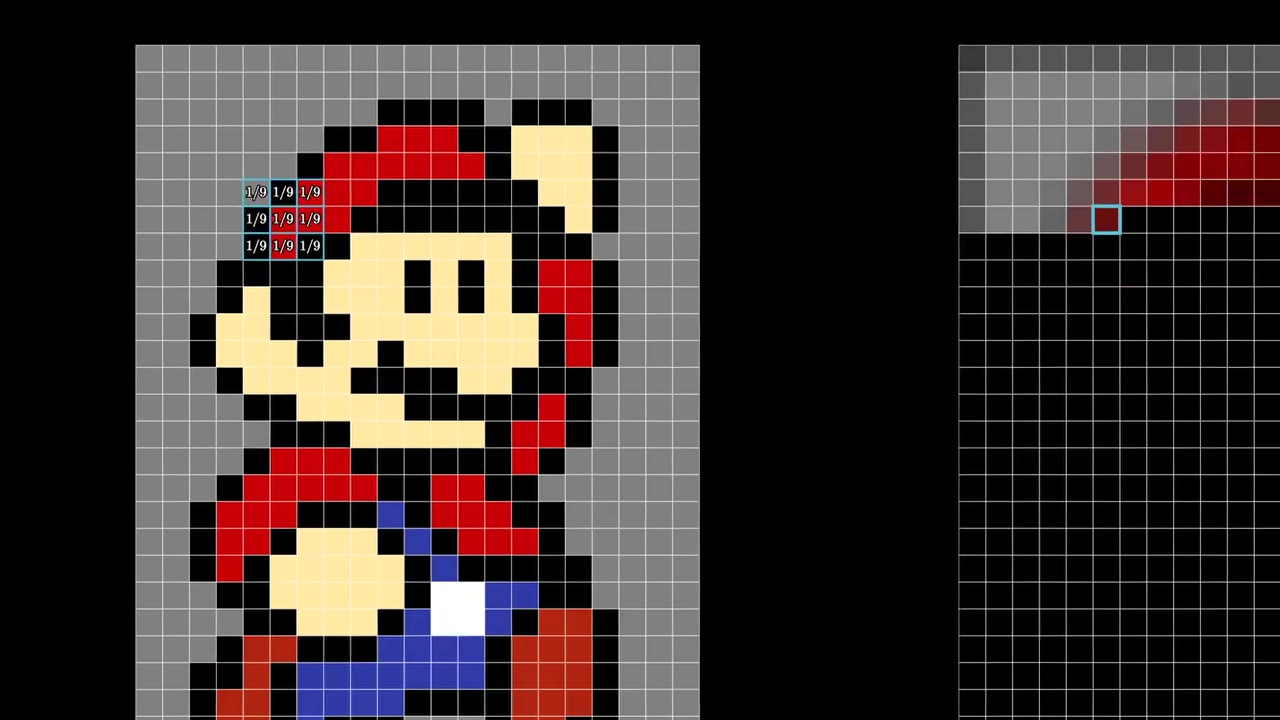
\includegraphics[width=\paperwidth,height=\paperheight]{3b1b_mario_kernel.jpg}}%
\begin{frame}[plain]
  \begin{tikzpicture}[remember picture, overlay]
    \fill[black, opacity=0.82] (current page.south west) rectangle
      ([yshift=2.55cm]current page.south east);
    \node[anchor=north west, text width=14.2cm, align=left, text=white]
      at ([shift={(0.75cm,2.35cm)}]current page.south west) {%
      {\Large\bfseries\color{armorange}Must watch}\par\vskip 3pt
      {\large 3Blue1Brown -
        \href{https://www.youtube.com/watch?v=KuXjwB4LzSA}{\color{white}\underline{But what is a
        convolution?}}}\par\vskip 3pt
      {\small 23 minutes, beautifully animated: sliding sums, dice, moving averages, image blur
      and edge kernels - this lecture's Section 2 - plus why the fast Fourier transform makes
      convolution fast.}};
    \node[anchor=north east, font=\tiny, text=white!75]
      at ([shift={(-0.2cm,-0.15cm)}]current page.north east) {3Blue1Brown (2022)};
  \end{tikzpicture}
\end{frame}}

% ================================================================
\section{Why dense nets are the wrong tool for images}

\begin{frame}[plain]
  \vfill
  \begin{center}
    {\Large\color{popblue}\textbf{Images are not feature vectors}}\\[0.9em]
    \begin{minipage}{0.82\textwidth}\centering\small
      A dense net treats a photo as a bag of unrelated numbers. That throws away the one
      thing images have: structure.
    \end{minipage}
  \end{center}
  \vfill
\end{frame}

% 2026-09-22: the three colour frames (cones / RGB / HSV) were folded into this one recap -
% deck [33] Color Spaces taught all three on 2026-08-20. Originals: git show 6f0f7cd:<this file>.
\begin{frame}{Color, recalled from [33]}
  \small
  [33] did the physics: three cone types, so a pixel is \textbf{three numbers}
  $(R, G, B)$, each $0$ to $255$ (HSV re-coordinatizes the same pixel - it returns in
  HW1b). Today only the \textbf{shape} matters: a color photo is \textbf{three stacked
  grids}, one per channel - a $3 \times H \times W$ block of numbers.
  \begin{center}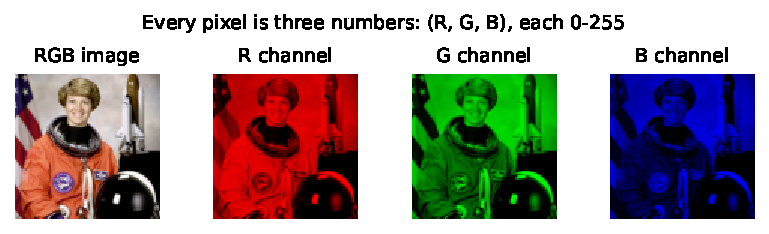
\includegraphics[width=0.96\linewidth]{rgb_channels.pdf}\end{center}
  \vskip -2pt
  \fcolorbox{armblue}{armblue!8}{\parbox{0.97\linewidth}{\small
    Hold on to "stacked grids". In Section 4 the stack depth becomes a conv layer's
    \textbf{input channels} - and every conv layer then builds a stack of its own.}}
  \vskip 3pt
  {\scriptsize\color{gray} Our test photo: astronaut Eileen Collins (NASA, public domain). For
  decades the field's standard test image was "Lena", a 1972 Playboy scan; IEEE stopped
  accepting it in papers in 2024, and photos like this one replaced it.}
\end{frame}

\begin{frame}{An image is a grid of numbers}
  \begin{columns}[T]
    \column{0.42\textwidth}
    A grayscale image is \textbf{one matrix}: each entry is a pixel intensity, $0$ (black)
    to $255$ (white).
    \vskip 6pt
    RGB or HSV, color is three stacked grids. From here we work in \textbf{grayscale} - one
    matrix - so the convolution mechanics stay 2D; channels return in Section 4.
    \vskip 6pt
    \fcolorbox{armblue}{armblue!8}{\parbox{0.95\linewidth}{\small
      To a computer there is no "image" - only a grid of numbers.}}
    \column{0.58\textwidth}
    \begin{center}
      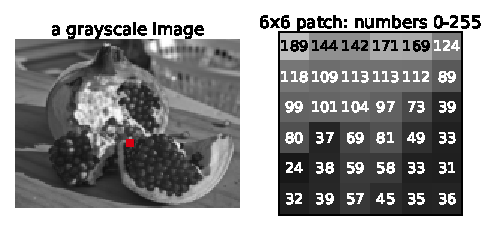
\includegraphics[width=\linewidth]{image_numbers.pdf}
    \end{center}
  \end{columns}
\end{frame}

\begin{frame}{An image is a function}
  \begin{columns}[T]
    \column{0.32\textwidth}
    Read the grid as a \textbf{function} $f(x,y)$: position in, intensity out.
    \vskip 6pt
    Walk along one horizontal line: $f$ is flat on uniform regions, a \textbf{ramp} across a
    gradient, and a \textbf{jump} at an edge.
    \vskip 6pt
    \fcolorbox{armblue}{armblue!8}{\parbox{0.95\linewidth}{\small
      An edge is where $f$ changes fast. That single idea is how we will detect edges.}}
    \column{0.68\textwidth}
    \begin{center}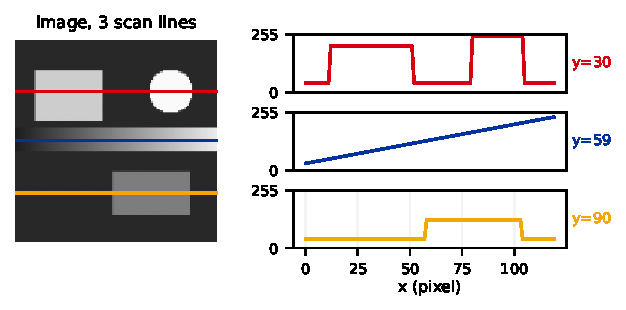
\includegraphics[width=\linewidth]{image_as_function.pdf}\end{center}
  \end{columns}
\end{frame}

\begin{frame}{An MLP cannot see structure}
  \begin{columns}[T]
    \column{0.40\textwidth}
    Flattening a photo into a $150{,}528$-vector hands the pixels to the net in \emph{some}
    order - but a dense layer treats every order the same.
    \vskip 6pt
    Shuffle the pixels with one fixed permutation and an MLP learns it \emph{exactly as
    well}. To us, one is a pomegranate and the other is noise.
    \vskip 6pt
    \fcolorbox{armred}{armred!8}{\parbox{0.95\linewidth}{\small
      Nearby pixels are related; far-apart ones usually are not. A dense layer knows none
      of this.}}
    \column{0.60\textwidth}
    \begin{center}
      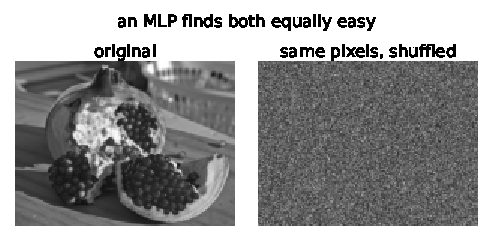
\includegraphics[width=\linewidth]{pixel_shuffle.pdf}
    \end{center}
  \end{columns}
\end{frame}

\begin{frame}{Two wishes}
  We want a layer that builds in what we know about images:
  \vskip 8pt
  \begin{enumerate}
    \item \textbf{Locality.} Detect a small pattern (an edge, a corner) from a small
      neighborhood of pixels - not from the whole image at once.
    \item \textbf{Reuse.} A detector that is useful in one corner is useful everywhere. A
      cat in the corner is still a cat.
  \end{enumerate}
  \vskip 4pt
  \small Wish 2 buys a property with a technical name, \textbf{translation equivariance}:
  shift the input, and the detector's output map shifts by the same amount. In 1D, with
  kernel $(1,2,3)$: input $(0,0,1,0,0) \to (3,2,1)$; move the spike one step right,
  $(0,0,0,1,0) \to (0,3,2)$ - the same response, one step later.
  \normalsize
  \vskip 10pt
  \fcolorbox{armblue}{armblue!8}{\parbox{0.97\linewidth}{
      These two wishes - \textbf{locality} and \textbf{weight reuse} - \emph{are} the
      convolutional layer. The rest of this lecture is just spelling them out.}}
\end{frame}

% 2026-09-22 addition: the biological origin of both wishes (web-verified: Hubel & Wiesel
% 1959/1962, Nobel 1981; Fukushima's neocognitron 1980 named its S/C-cells after them).
\begin{frame}{Nature had the same two wishes}
  \small
  1959-62: \textbf{David Hubel} and \textbf{Torsten Wiesel} recorded single neurons in a
  cat's visual cortex while showing it bars of light (Nobel Prize, 1981). Two kinds of
  cell turned up:
  \vskip 6pt
  \begin{center}
    \begin{tabular}{p{0.19\linewidth} p{0.44\linewidth} p{0.26\linewidth}}
      \textbf{Cell} & \textbf{Fires when...} & \textbf{In a CNN}\\
      \hline
      \textbf{simple} & an edge at \emph{one orientation} appears in \emph{one small
        patch} of the visual field & a conv kernel (local, oriented - a Sobel)\\[3pt]
      \textbf{complex} & that same edge appears \emph{anywhere} in a somewhat larger
        region & pooling over nearby detectors\\
    \end{tabular}
  \end{center}
  \vskip 6pt
  The brain tiles the whole visual field with copies of the same small detectors -
  locality \emph{and} reuse.
  \vskip 6pt
  \fcolorbox{armblue}{armblue!8}{\parbox{0.97\linewidth}{\small
    Convolution and pooling were not invented from scratch: they are an engineer's copy
    of the first two stages of the visual cortex. The next slide traces that copy.}}
\end{frame}

\begin{frame}{Where CNNs came from}
  Convolutional nets are not new - biology, then one idea, then ten years of engineering:
  \vskip 6pt
  \begin{itemize}
    \item \textbf{1980 - Kunihiko Fukushima's neocognitron.} Layers of "S-cells" and
      "C-cells", named after Hubel and Wiesel's simple and complex cells: convolution and
      pooling, stacked. But no backprop - its detectors were not trained end to end.
    \item \textbf{1989-1998 - one project at Bell Labs, ten years long.} Yann LeCun and
      colleagues train such layers \textbf{with backpropagation} to read \textbf{handwritten
      ZIP codes} on U.S. mail (1989). They refine the design version after version - LeNet-1
      to \textbf{LeNet-5} - until it reads bank checks commercially, and in \textbf{1998}
      write the whole decade up in one paper (LeCun, Bottou, Bengio \& Haffner), with the
      \textbf{MNIST} digit benchmark.
  \end{itemize}
  {\small Not two attempts: 1989 is the first working version, 1998 the polished one.
  Everything in this lecture descends from it.}
  \vskip 6pt
  \fcolorbox{paramgreen}{paramgreen!8}{\parbox{0.97\linewidth}{\small
      Same recipe then and now: local filters, shared weights, pooling, a dense head. Later
      lectures just make it bigger, deeper, and trained on far more data.}}
\end{frame}

\begin{frame}{CNNs in the wild}
  \begin{columns}[T]
    \column{0.5\textwidth}
    \begin{center}
      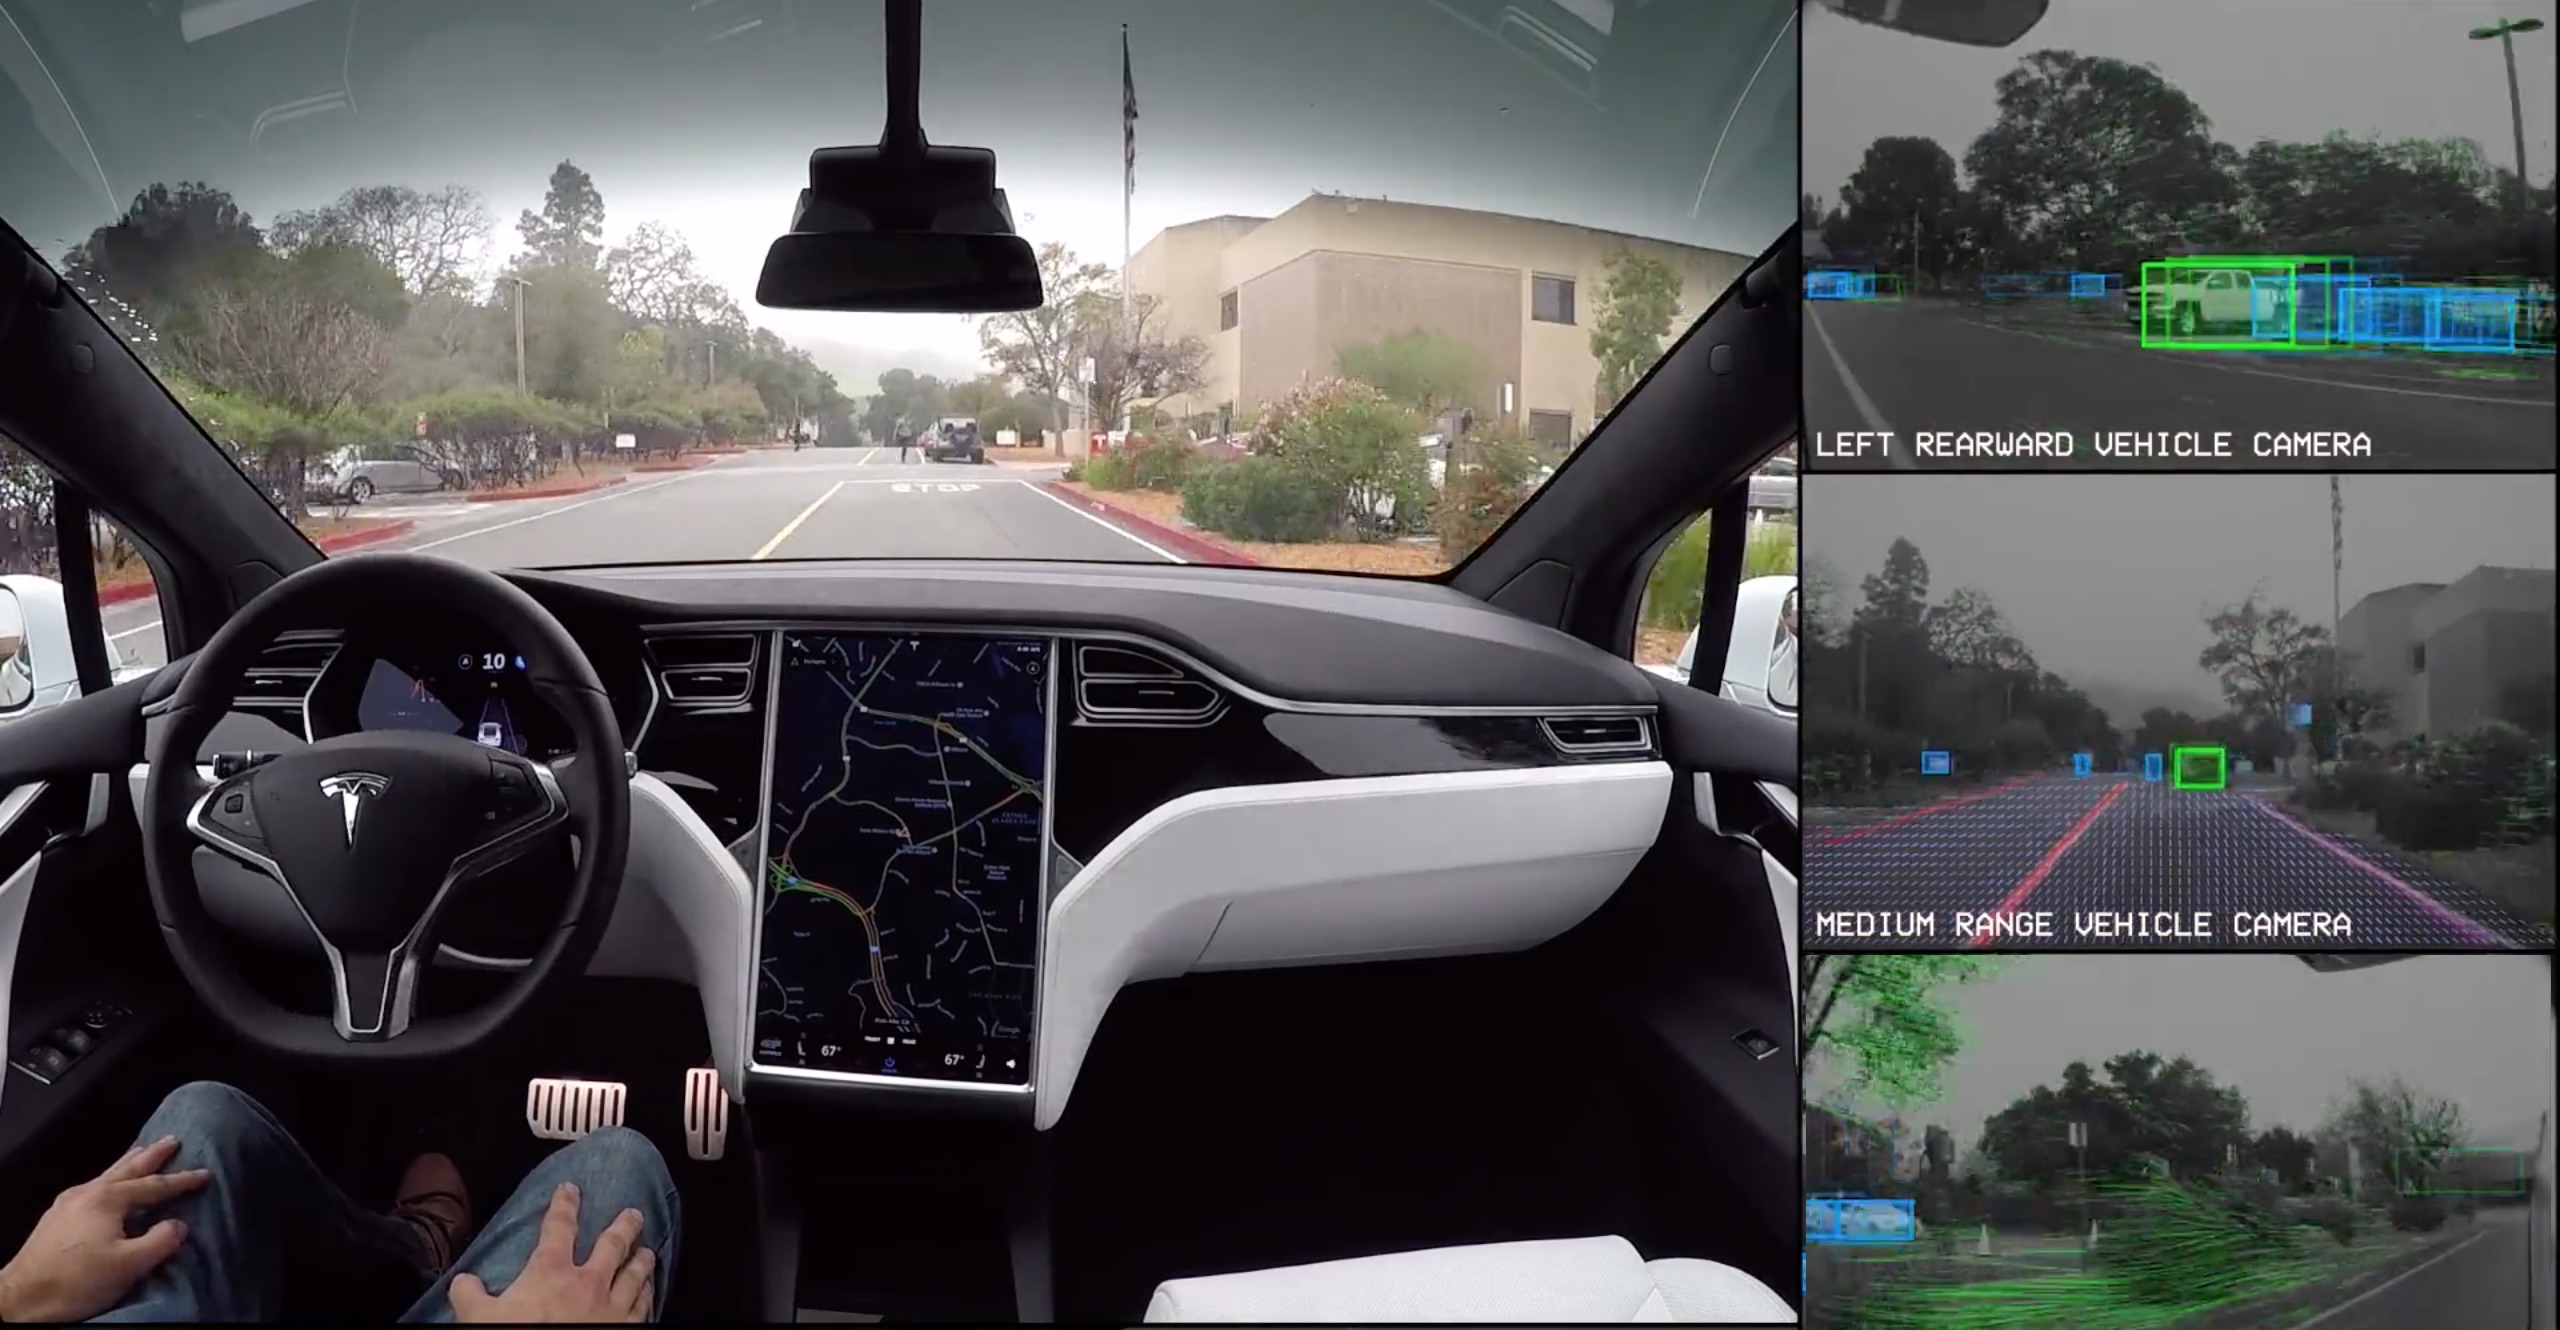
\includegraphics[height=0.25\textheight]{tesla_autopilot.jpg}\\[1pt]
      {\scriptsize self-driving perception}
    \end{center}
    \vskip 2pt
    \begin{center}
      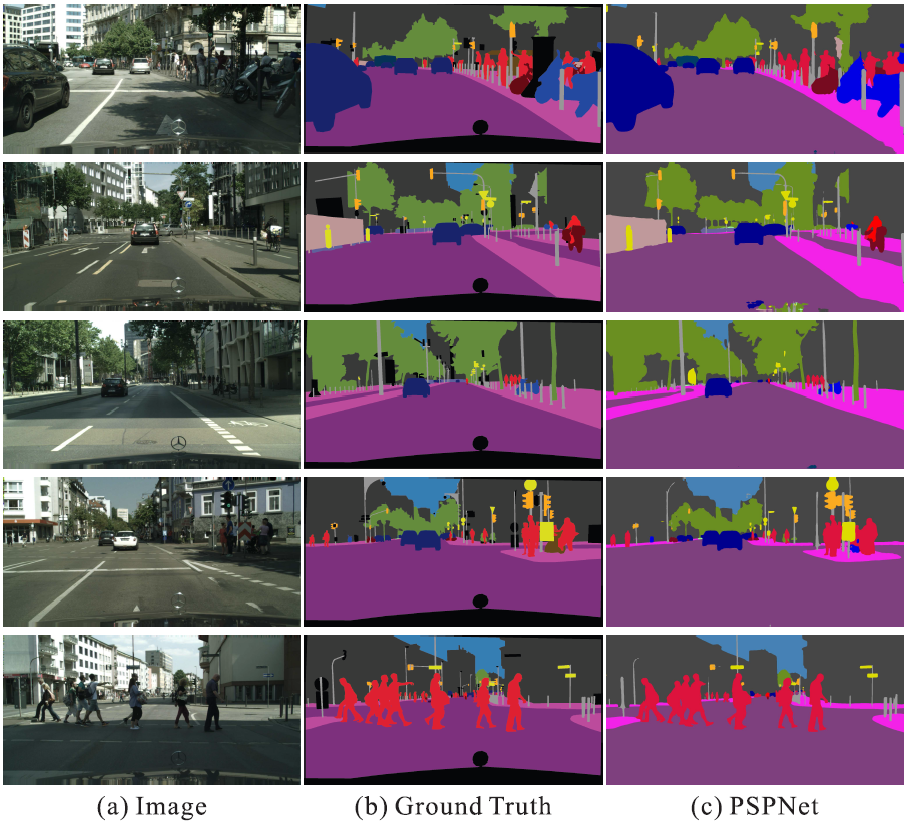
\includegraphics[height=0.25\textheight]{cityscapes_visual.png}\\[1pt]
      {\scriptsize semantic segmentation}
    \end{center}
    \column{0.5\textwidth}
    \begin{center}
      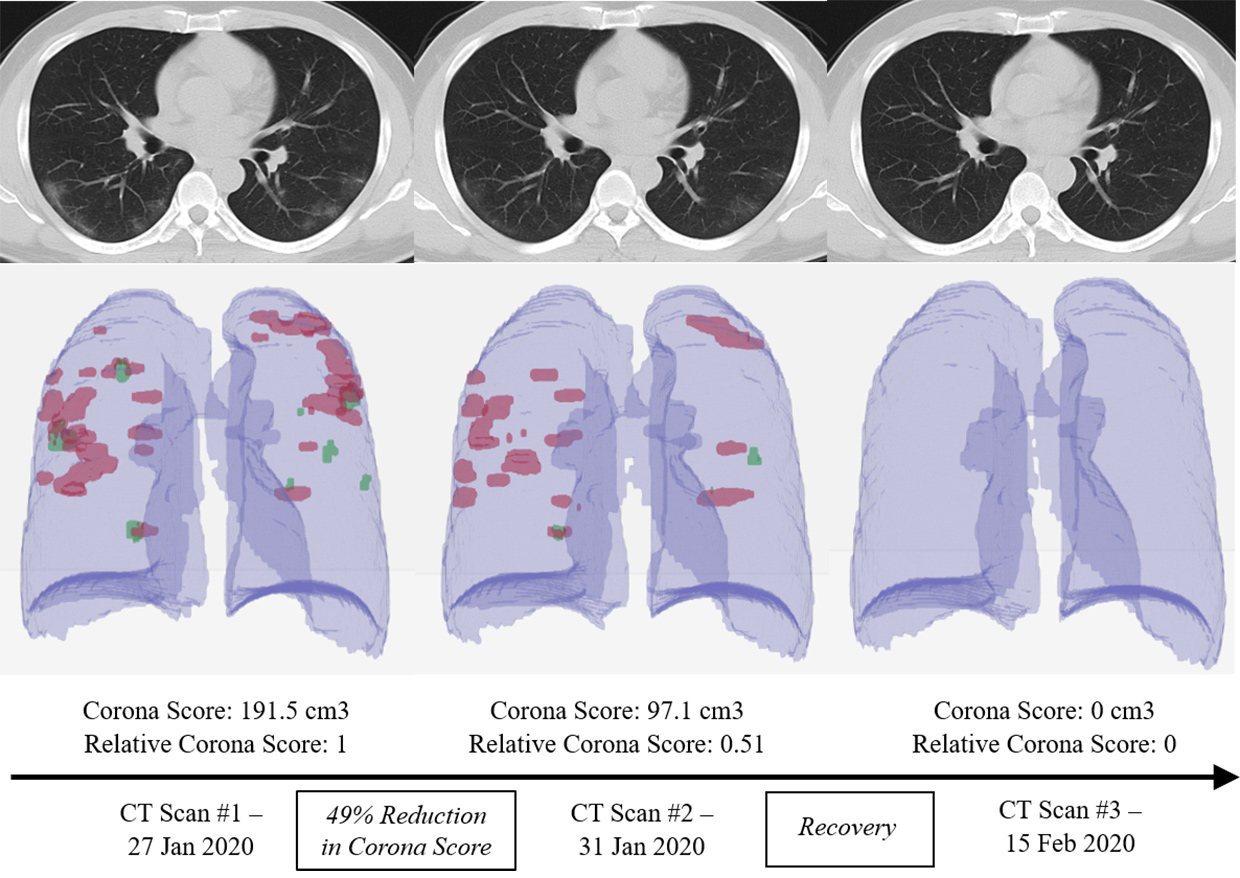
\includegraphics[height=0.25\textheight]{coronatrack.jpeg}\\[1pt]
      {\scriptsize medical CT screening}
    \end{center}
    \vskip 2pt
    \begin{center}
      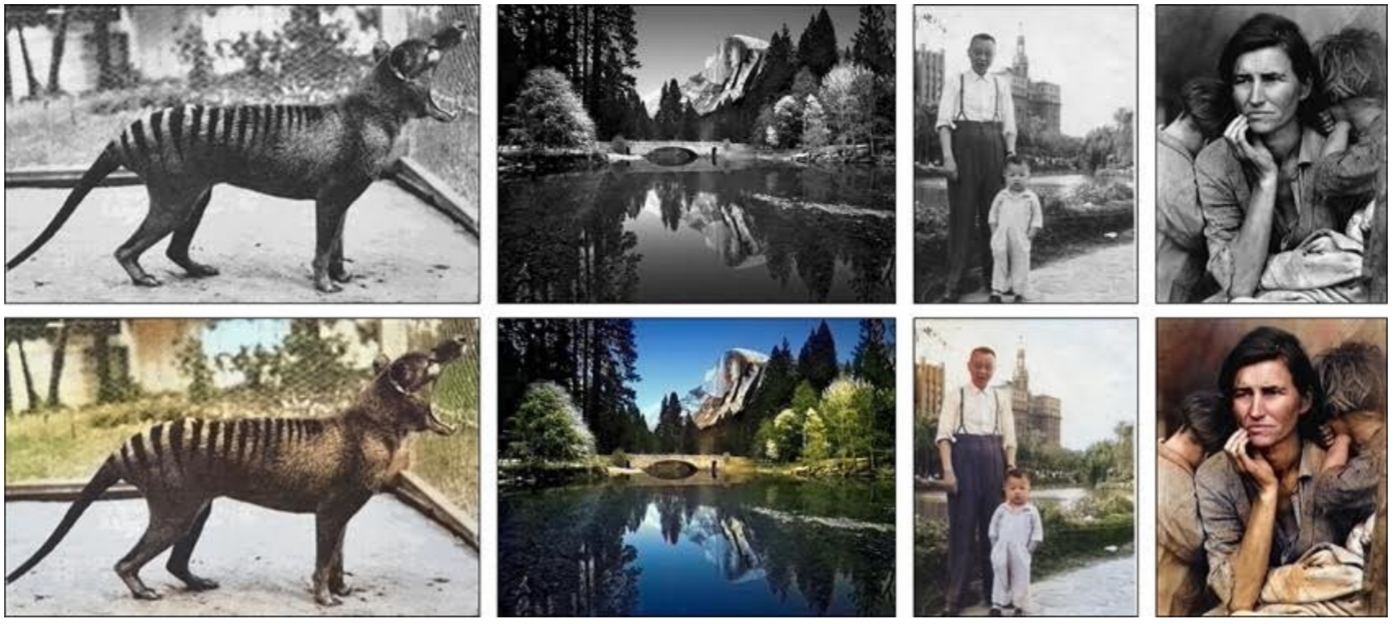
\includegraphics[height=0.25\textheight]{colorization.png}\\[1pt]
      {\scriptsize image colorization}
    \end{center}
  \end{columns}
  \vskip 4pt
  \begin{center}\scriptsize\color{gray}
    All built from this chapter's machinery.\quad Images: LMU I2DL (slds-lmu), CC BY 4.0.
  \end{center}
\end{frame}

% ================================================================
\section{The convolution operation}

\begin{frame}[plain]
  \vfill
  \begin{center}
    {\Large\color{popblue}\textbf{The convolution operation}}\\[0.9em]
    \begin{minipage}{0.82\textwidth}\centering\small
      Slide a small window across the input; at each stop, take a dot product.
    \end{minipage}
  \end{center}
  \vfill
\end{frame}

\begin{frame}{Start in 1D: a sliding dot product}
  \begin{columns}[T]
    \column{0.46\textwidth}
    Take a length-3 kernel $\mathbf{w}=(w_1,w_2,w_3)$ and slide it along a sequence. Each
    output is the dot product of the kernel with the window under it.
    \vskip 6pt
    With $\mathbf{w}=(\tfrac13,\tfrac13,\tfrac13)$ this is exactly a \textbf{moving
    average}. Different weights detect different local patterns.
    \vskip 6pt
    \fcolorbox{armblue}{armblue!8}{\parbox{0.95\linewidth}{\small
      Same idea works on any sequence - audio, sensor traces, text. Convolution is a prior,
      not an image trick (more in [50]).}}
    \column{0.54\textwidth}
    \begin{center}
      \begin{tikzpicture}[font=\scriptsize, >=Latex,
        c/.style={draw, minimum size=0.6cm, inner sep=0}]
        \foreach \v/\i in {2/0,1/1,3/2,5/3,4/4,2/5,1/6}
          \node[c, fill=gray!8] (x\i) at (\i*0.62,1.4) {\v};
        \node[c, draw=armblue, very thick] at (1*0.62,1.4) {};
        \node[c, draw=armblue, very thick] at (2*0.62,1.4) {};
        \node[c, draw=armblue, very thick] at (3*0.62,1.4) {};
        \node[armblue] at (2*0.62,2.15) {\footnotesize kernel $(w_1,w_2,w_3)$};
        \foreach \v/\i in {2/0,3/1,4/2,3.7/3,2.3/4}
          \node[c, fill=paramgreen!12] (o\i) at (\i*0.62+0.62,0.2) {\v};
        \draw[->, armblue] (2*0.62,1.1) -- (2*0.62+0.0,0.5);
        \node at (2*0.62,-0.5) {\footnotesize output $=w_1(1)+w_2(3)+w_3(5)$};
      \end{tikzpicture}
    \end{center}
  \end{columns}
\end{frame}

\begin{frame}{The moving average is a convolution}
  \begin{columns}[T]
    \column{0.36\textwidth}
    Slide a box kernel $[\tfrac15,\tfrac15,\tfrac15,\tfrac15,\tfrac15]$ over a noisy signal:
    each output is the \textbf{average} of its neighbours, so the signal comes out
    \textbf{smoothed}.
    \vskip 6pt
    Blur, smooth, denoise - all the same sliding-and-summing. Different weights give
    different effects.
    \column{0.64\textwidth}
    \begin{center}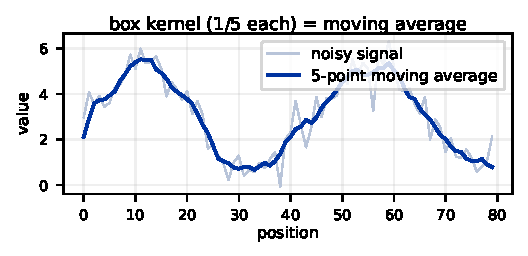
\includegraphics[width=\linewidth]{moving_average.pdf}\end{center}
  \end{columns}
\end{frame}

\begin{frame}{Aside: convolution lives in probability too}
  \begin{columns}[T]
    \column{0.34\textwidth}
    Roll \textbf{two dice} and add them. The distribution of the \emph{sum} is the
    \textbf{convolution} of the two single-die distributions.
    \vskip 6pt
    Two flat uniforms slide across each other and their overlap is summed - giving the
    triangle that peaks at $7$.
    \vskip 6pt
    \fcolorbox{armblue}{armblue!8}{\parbox{0.95\linewidth}{\small
      Same operation, different field. Convolution is a general tool, not an image trick.}}
    \vskip 4pt
    {\scriptsize\color{gray} It lives in frequency space too - see the appendix.}
    \column{0.66\textwidth}
    \begin{center}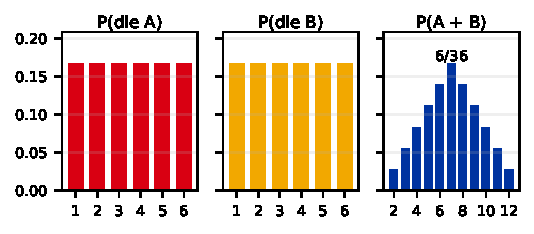
\includegraphics[width=\linewidth]{dice_conv.pdf}\end{center}
  \end{columns}
\end{frame}

% 2026-10-01: the 4-frame Fourier aside (Taylor -> Fourier, spectrum, convolution theorem,
% blur/edges as frequency filters) moved to the appendix at the end (instructor request).

\begin{frame}{2D convolution, by hand}
  \begin{columns}[T]
    \column{0.5\textwidth}
    Input $I$, kernel $W$ ($2\times2$). Slide $W$ over $I$; each output cell is the dot
    product with the $2\times2$ window under it.
    \[
      I=\begin{bmatrix}1&2&0\\3&1&1\\0&2&4\end{bmatrix}\quad
      W=\begin{bmatrix}0&1\\2&2\end{bmatrix}
    \]
    Top-left window $\begin{bmatrix}1&2\\3&1\end{bmatrix}$:
    \[
      s_{11}=1{\cdot}0+2{\cdot}1+3{\cdot}2+1{\cdot}2 = 10
    \]
    In one line:
    \[
      s_{ij}=\sum_{m,n} I(i{+}m{-}1,\,j{+}n{-}1)\,w(m,n)
    \]
    \column{0.5\textwidth}
    Repeat for all four positions:
    \[
      S=\begin{bmatrix}10&4\\5&13\end{bmatrix}
    \]
    \vskip 2pt
    \fcolorbox{popblue}{popblue!6}{\parbox{0.95\linewidth}{\small
      \textbf{Feature map} (or activation map): the output grid $S$. One number per position:
      how strongly the kernel's pattern is present \emph{there}. A kernel that detects
      vertical edges produces a map that lights up wherever the image has one.}}
    \vskip 4pt
    \fcolorbox{armblue}{armblue!8}{\parbox{0.95\linewidth}{\small
      A $2\times2$ kernel on a $3\times3$ input gives a $2\times2$ map. It
      \emph{shrinks} - we fix that with padding in Section 4.}}
  \end{columns}
\end{frame}

% 2026-10-01: figure redrawn at its slide size (embedded at its native 4.87 in, so its labels are
% 8-12 pt) with an orange sliding window - the dark-blue one vanished on dark cells (instructor).
\begin{frame}{Convolution, step by step}
  Watch the kernel slide. At each stop the output cell is a \textbf{weighted average} of the
  window under it - here a \emph{Gaussian blur} (center weighted most, divided by $16$), so
  the patch comes out \emph{smoothed}. Light cells are high values. \textbf{(Click to advance.)}
  \vskip 2pt
  \begin{center}
    \only<1>{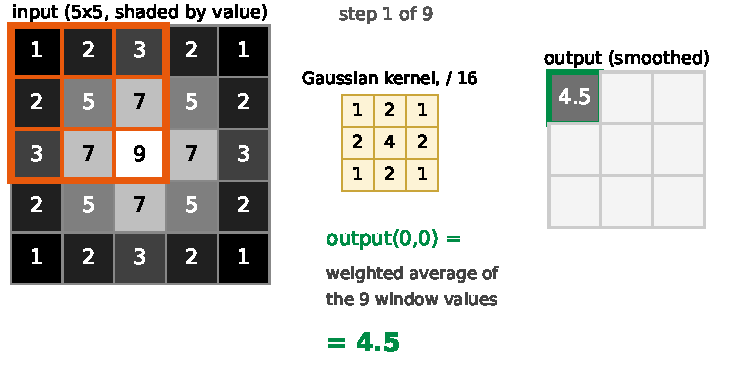
\includegraphics[width=4.87in]{conv_anim_0.pdf}}%
    \only<2>{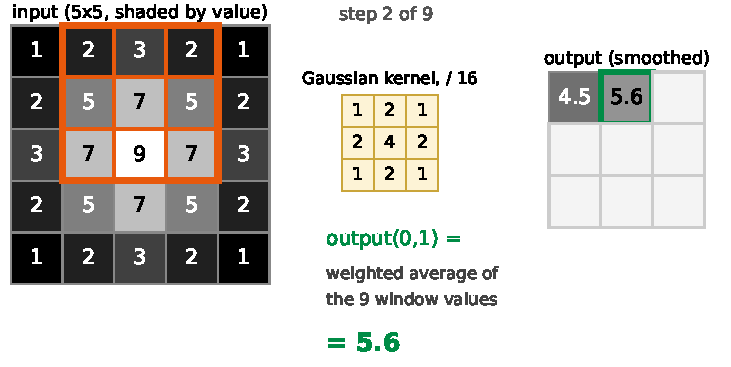
\includegraphics[width=4.87in]{conv_anim_1.pdf}}%
    \only<3>{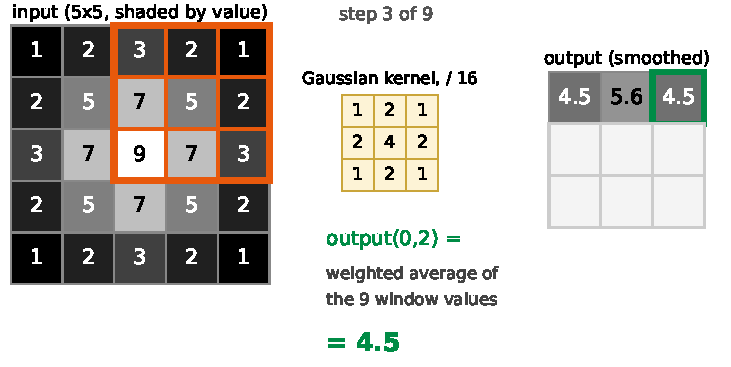
\includegraphics[width=4.87in]{conv_anim_2.pdf}}%
    \only<4>{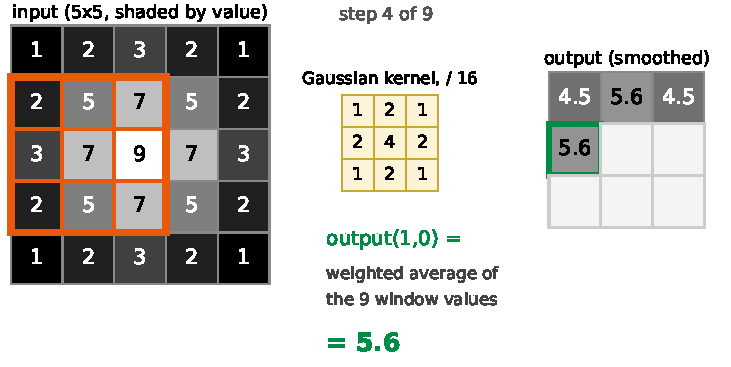
\includegraphics[width=4.87in]{conv_anim_3.pdf}}%
    \only<5>{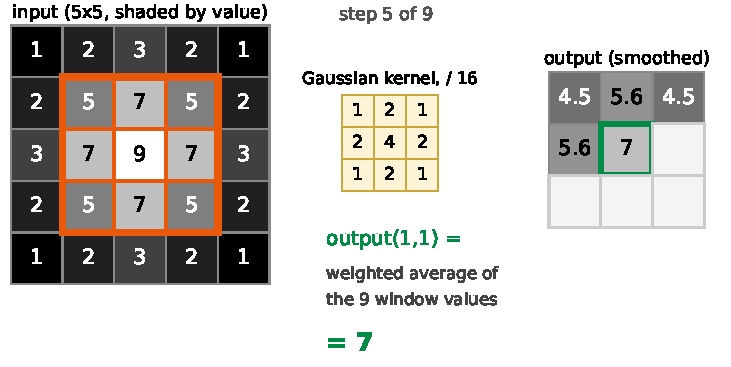
\includegraphics[width=4.87in]{conv_anim_4.pdf}}%
    \only<6>{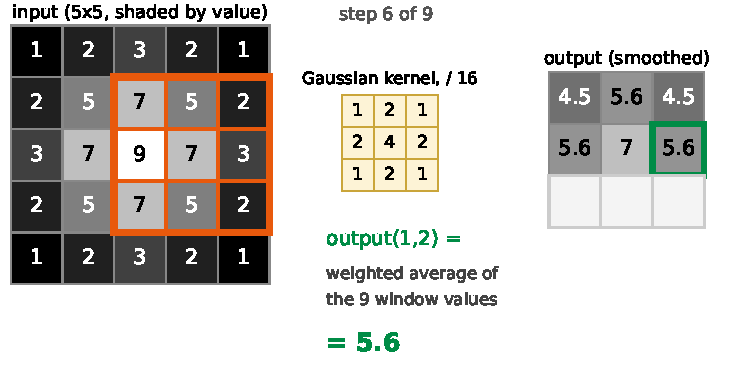
\includegraphics[width=4.87in]{conv_anim_5.pdf}}%
    \only<7>{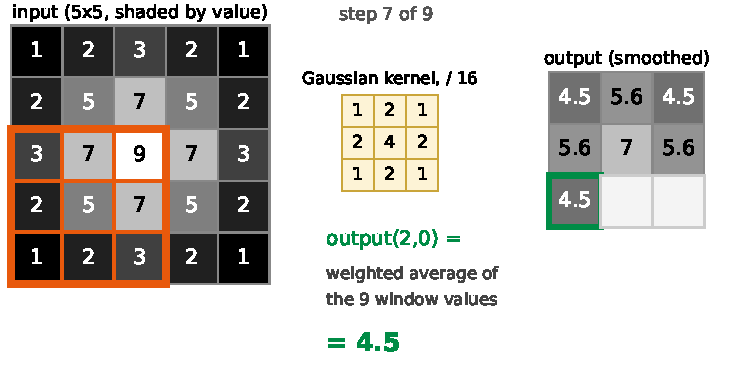
\includegraphics[width=4.87in]{conv_anim_6.pdf}}%
    \only<8>{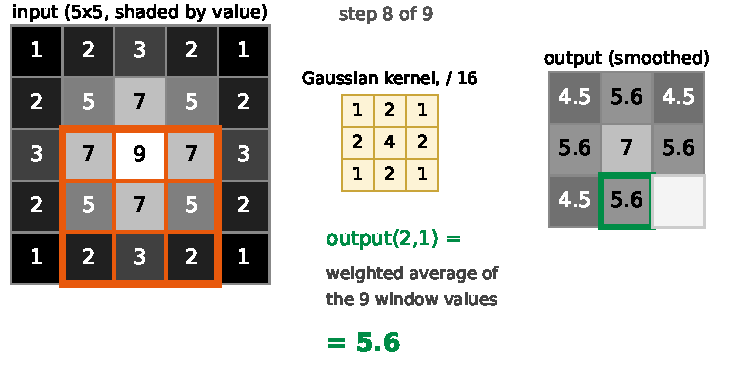
\includegraphics[width=4.87in]{conv_anim_7.pdf}}%
    \only<9>{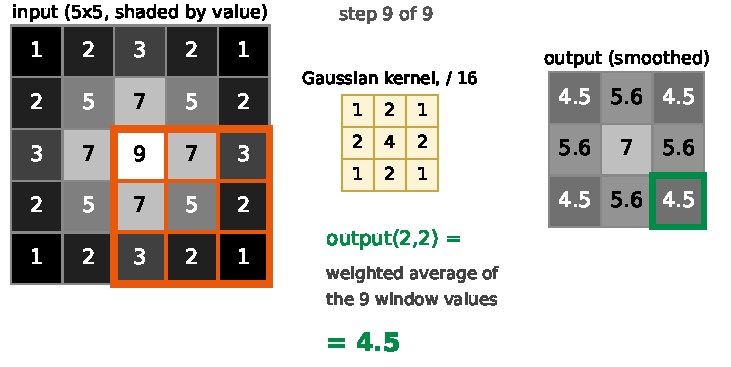
\includegraphics[width=4.87in]{conv_anim_8.pdf}}%
  \end{center}
\end{frame}

\begin{frame}{The kernel zoo: hand-designed filters}
  \begin{columns}[T]
    \column{0.30\textwidth}
    The same $3\times3$ machinery, seven classic kernels. \textbf{Predict} before you look:
    \vskip 4pt
    {\footnotesize
    box blur $=\tfrac19\begin{bmatrix}1&1&1\\1&1&1\\1&1&1\end{bmatrix}$}
    \vskip 3pt
    {\footnotesize
    Sobel X $=\begin{bmatrix}-1&0&1\\-2&0&2\\-1&0&1\end{bmatrix}$}
    \pause
    \vskip 6pt
    \fcolorbox{armblue}{armblue!8}{\parbox{0.95\linewidth}{\small
      Box blur averages a neighborhood; Sobel X responds to \emph{vertical} edges. Same
      operation, different numbers.}}
    \column{0.70\textwidth}
    \begin{center}
      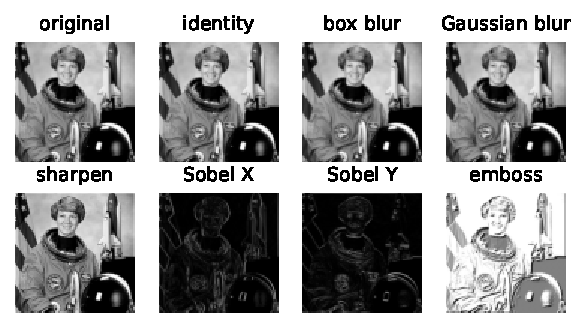
\includegraphics[width=\linewidth]{kernel_zoo.pdf}\\[2pt]
      \href{https://setosa.io/ev/image-kernels/}{\beamergotobutton{try your own kernel:
      Image Kernels, explained visually}}
    \end{center}
  \end{columns}
\end{frame}

% 2026-10-02 addition (instructor: "a few frames showing a zoo of kernels, values nicely
% visualized, include Gabor"). Figures: py_src/kernel_gallery.py. The Gabor frame sits after
% "From a difference to Sobel", where oriented edge detectors have been explained.
\begin{frame}{Kernel zoo, up close (1): averaging}
  \small
  \textbf{Kernel}, \textbf{filter}, \textbf{convolution matrix} (GIMP's menu name), mask: four
  names for one small grid of numbers. Each grid below shows its real values -
  \textcolor{armred}{red $>0$}, white $=0$, \textcolor{armblue}{blue $<0$}:
  \par\vskip 2pt{\centering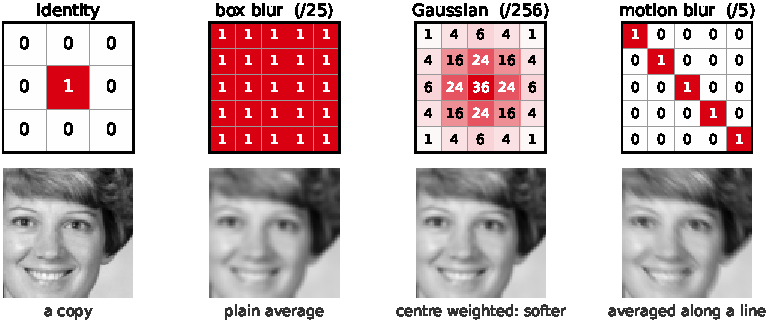
\includegraphics{kernel_gallery_blur.pdf}\par}
  \fcolorbox{armblue}{armblue!8}{\parbox{0.97\linewidth}{\small
    All four have weights $\ge 0$ that \textbf{sum to 1}: a weighted average. Brightness stays,
    detail goes - and a bigger kernel blurs more.}}
\end{frame}

\begin{frame}{Kernel zoo, up close (2): edges and sharpening}
  \small
  Negative weights \emph{subtract}: the kernel compares a pixel with its neighbours. (In the two
  signed maps, gray $=0$, white $>0$, black $<0$.)
  \par\vskip 2pt{\centering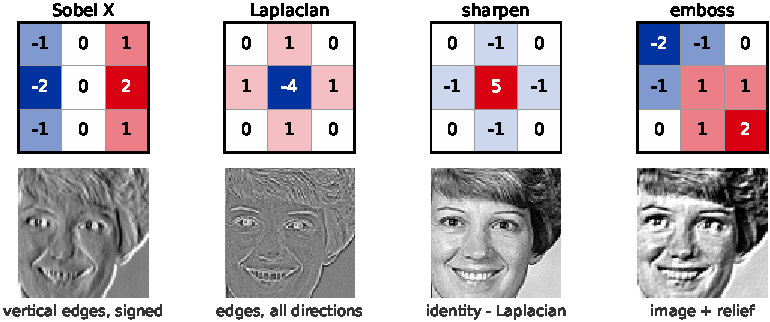
\includegraphics{kernel_gallery_edges.pdf}\par}
  \fcolorbox{armblue}{armblue!8}{\parbox{0.97\linewidth}{\small
    Sobel X and the Laplacian \textbf{sum to 0}: a flat patch gives 0, only \emph{change}
    answers - an edge detector (why: next slides). Sharpen and emboss sum to 1: the image
    itself, plus its edges.}}
\end{frame}

\begin{frame}{Why do those numbers find edges?}
  \begin{columns}[T]
    \column{0.46\textwidth}
    An edge is where intensity \textbf{changes fast} - a jump in $f$. "Fast change" is
    precisely what a \textbf{derivative} measures.
    \vskip 6pt
    On a pixel grid the derivative is a \textbf{difference of neighbours}:
    \[
      f'(x)\ \approx\ \frac{f(x{+}1)-f(x)}{1},
    \]
    which is just $f(x{+}1)-f(x)$: near zero on flat regions, large at an edge.
    \column{0.54\textwidth}
    \begin{center}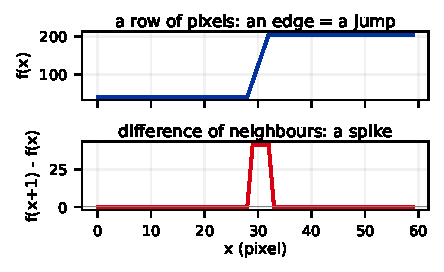
\includegraphics[width=\linewidth]{edge_1d.pdf}\end{center}
  \end{columns}
\end{frame}

\begin{frame}{The simplest edge detector is a kernel}
  A \emph{centered} difference looks one step each way:
  \[
    f(x{+}1)-f(x{-}1)\quad\Longleftrightarrow\quad\text{kernel }[\,{-}1\ \ 0\ \ 1\,].
  \]
  Slide $[{-}1\ 0\ 1]$ across a row and you read off its horizontal derivative - large
  wherever a \textbf{vertical} edge sits. Its transpose finds horizontal edges.
  \vskip 8pt
  \fcolorbox{armblue}{armblue!8}{\parbox{0.97\linewidth}{\small
      An edge detector is just a tiny kernel. The calculus hands us the numbers - no guessing
      required.}}
\end{frame}

\begin{frame}{From a difference to Sobel}
  \begin{columns}[T]
    \column{0.40\textwidth}
    \small
    A bare $[{-}1\ 0\ 1]$ is \textbf{noisy} - it fires on every speckle. Fix it by
    \textbf{averaging} down the column while differencing across the row:
    \[
      \underbrace{\begin{bmatrix}1\\2\\1\end{bmatrix}}_{\text{smooth}}
      \underbrace{[{-}1\ 0\ 1]}_{\text{difference}}
      =\begin{bmatrix}-1&0&1\\-2&0&2\\-1&0&1\end{bmatrix}
    \]
    That is \textbf{Sobel X}; its transpose is Sobel Y. Together they give the gradient -
    edge strength and direction.
    \column{0.60\textwidth}
    \begin{center}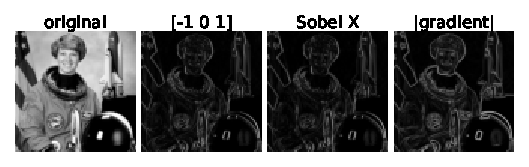
\includegraphics[width=\linewidth]{sobel_build.pdf}\end{center}
  \end{columns}
  \vskip 2pt
  \fcolorbox{armorange}{armorange!12}{\parbox{0.97\linewidth}{\small
      A \textbf{spatially separable} kernel (column $\times$ row - two 1D passes, not one 2D).
      Filters like these ran computer vision for 30 years, each hand-designed by an expert.
      Hold that thought.}}
\end{frame}

\begin{frame}{Kernel zoo, up close (3): Gabor filters}
  \small
  A \textbf{Gabor filter} is a Gaussian blob times a cosine wave: it answers to stripes of
  \emph{one} angle and \emph{one} width. $21\times21$ values each - read the colours:
  \par\vskip 2pt{\centering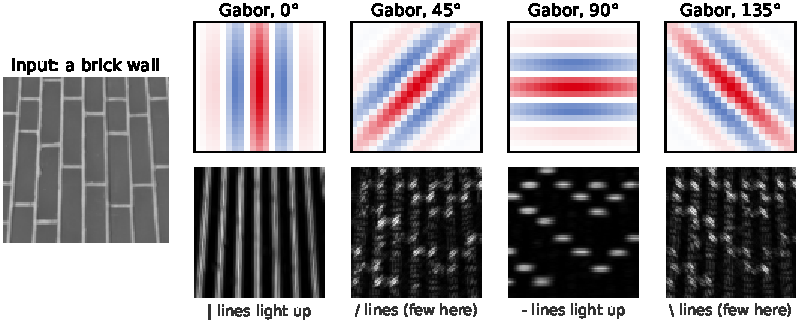
\includegraphics[width=5.0in]{kernel_gallery_gabor.pdf}\par}
  \fcolorbox{armblue}{armblue!8}{\parbox{0.97\linewidth}{\small
    $g=e^{-(x'^2+\gamma^2y'^2)/2\sigma^2}\cos(2\pi x'/\lambda)$, $(x',y')$ rotated by
    $\theta$. Cat visual-cortex cells fit this shape (Jones \& Palmer, 1987); CNNs trained on
    ImageNet grow Gabor-like first layers on their own ([49]).}}
\end{frame}

\begin{frame}{The punchline: a CNN designs its own kernels}
  A kernel is just a grid of numbers. Those numbers are \textbf{weights}.
  \vskip 6pt
  So instead of an expert choosing $\begin{bmatrix}-1&0&1\\-2&0&2\\-1&0&1\end{bmatrix}$, we
  let \textbf{gradient descent} choose every entry - exactly as it has tuned every weight
  since [02]. The loss decides which detectors are worth having.
  \vskip 8pt
  \fcolorbox{armblue}{armblue!8}{\parbox{0.97\linewidth}{
      \textbf{Misconception, pre-empted.} CNN kernels are \emph{not} hand-engineered. They
      are \emph{learned}. That is the whole point: we stop hand-designing feature detectors
      ([26]) and let the network learn its own representation ([41\_1]).}}
\end{frame}

\begin{frame}{A kernel is a neuron you already know}
  \begin{columns}[T]
    \column{0.55\textwidth}
    A $3\times3$ kernel has \textbf{$9$ weights $+$ $1$ bias}. At each position it computes
    \[
      \textstyle z=\sum_{k} w_k x_k + b,\qquad a=\phi(z)
    \]
    an affine map followed by an activation - \textbf{exactly the [41\_1] neuron}.
    \vskip 6pt
    Two differences only: it is wired to a small \emph{patch}, not the whole image; and the
    \emph{same} neuron is reused at every location.
    \vskip 6pt
    \fcolorbox{paramgreen}{paramgreen!8}{\parbox{0.95\linewidth}{\small
      Nothing about training changes. One neuron, reused at every pixel.}}
    \column{0.45\textwidth}
    \begin{center}
      \begin{tikzpicture}[font=\scriptsize, >=Latex]
        \foreach \i in {0,1,2}\foreach \j in {0,1,2}
          \node[draw, minimum size=0.42cm, fill=armblue!10] (p\i\j) at (\j*0.46,-\i*0.46) {};
        \node[circle, draw, fill=armorange!16, minimum size=0.8cm] (n) at (3.0,-0.46) {$\Sigma,\phi$};
        \foreach \i in {0,1,2}\foreach \j in {0,1,2}
          \draw[gray!55, ->] (p\i\j) -- (n);
        \node[draw, minimum size=0.5cm, fill=paramgreen!12] (o) at (4.4,-0.46) {};
        \draw[->, thick] (n) -- (o);
        \node at (1.0,-1.65) {\footnotesize $3{\times}3$ patch};
        \node at (4.4,-1.2) {\footnotesize output pixel};
      \end{tikzpicture}
    \end{center}
  \end{columns}
\end{frame}

\begin{frame}{Footnote: convolution vs cross-correlation}
  Purists note: true \emph{convolution} flips the kernel before the dot product; what we
  (and every deep-learning framework) just did, \emph{without} flipping, is technically
  \textbf{cross-correlation}.
  \vskip 8pt
  PyTorch's \texttt{nn.Conv2d} computes cross-correlation and calls it convolution.
  \vskip 8pt
  \fcolorbox{armblue}{armblue!8}{\parbox{0.97\linewidth}{\small
      It makes no difference in practice: the kernel is \emph{learned} either way, so it
      would just learn the flipped version.}}
\end{frame}

% ================================================================
\section{Why convolution is the right prior}

\begin{frame}[plain]
  \vfill
  \begin{center}
    {\Large\color{popblue}\textbf{Why convolution is the right prior}}\\[0.9em]
    \begin{minipage}{0.82\textwidth}\centering\small
      Locality and reuse do not just feel right - they collapse the parameter count.
    \end{minipage}
  \end{center}
  \vfill
\end{frame}

\begin{frame}{Sparse connectivity}
  \begin{columns}[T]
    \column{0.5\textwidth}
    A $3\times3$ input, a $2\times2$ kernel, a $2\times2$ output. Each output pixel wires
    only to the $2\times2$ patch it came from - its \textbf{receptive field}.
    \vskip 6pt
    Count the links: $4$ outputs $\times\,4$ inputs each $=\textbf{16}$. A dense layer would
    wire every output to all $9$ inputs: $9\times4=\textbf{36}$.
    \vskip 6pt
    \fcolorbox{armblue}{armblue!8}{\parbox{0.95\linewidth}{\small
      Locality alone already cuts the connections. And it scales: bigger images, far bigger
      savings.}}
    \column{0.5\textwidth}
    \begin{center}
      \begin{tikzpicture}[font=\scriptsize, >=Latex]
        \foreach \i in {0,1,2}\foreach \j in {0,1,2}
          \node[draw, minimum size=0.5cm, fill=gray!8] (i\i\j) at (\j*0.55,-\i*0.55) {};
        % highlight top-left 2x2 receptive field
        \foreach \i in {0,1}\foreach \j in {0,1}
          \node[draw=armblue, very thick, minimum size=0.5cm] at (\j*0.55,-\i*0.55) {};
        \foreach \i in {0,1}\foreach \j in {0,1}
          \node[draw, minimum size=0.5cm, fill=paramgreen!12] (o\i\j) at (2.7+\j*0.55,-0.28-\i*0.55) {};
        \foreach \i in {0,1}\foreach \j in {0,1}
          \draw[armblue!70, ->] (i\i\j) -- (o00);
        \node at (0.55,-1.75) {\footnotesize $2{\times}2$ patch};
        \node at (2.95,-1.75) {\footnotesize one output};
      \end{tikzpicture}
    \end{center}
  \end{columns}
\end{frame}

\begin{frame}{Parameter sharing}
  \begin{columns}[T]
    \column{0.42\textwidth}
    Those $16$ connections do not use $16$ different weights. Every output pixel uses the
    \emph{same} $4$ kernel weights - the kernel is \textbf{shared} across all positions.
    \vskip 6pt
    So: $4$ distinct weights, not $36$. Scale it up - a $100\times100\times3$ image, one
    $5\times5$ filter, same padding:
    \[
      \underbrace{5\cdot5\cdot3}_{75}\ \text{vs}\ \underbrace{300{,}000{,}000}_{\text{dense}}
    \]
    \column{0.58\textwidth}
    \begin{center}
      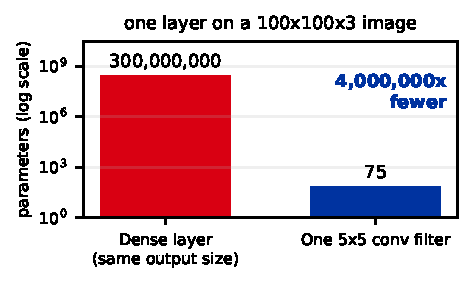
\includegraphics[width=\linewidth]{param_explosion.pdf}
    \end{center}
  \end{columns}
\end{frame}

% 2026-10-01 expansion (instructor: "expand on regularization"): the old single frame became
% two - the constrained-matrix picture (conv_as_matrix.py: 48 free weights vs 3) and the
% soft-vs-hard prior comparison. "Infinitely strong prior": Goodfellow, Bengio & Courville,
% Deep Learning (2016), Sec. 9.4 - web-checked 2026-10-01.
\begin{frame}{A conv layer is a dense layer with handcuffs}
  \small
  Write a 1D convolution the way we write a dense layer, $\mathbf{y} = W\mathbf{x}$: 8
  inputs, 6 outputs, kernel $(w_1, w_2, w_3)$. Row $i$ holds the kernel, shifted $i$ steps:
  \vskip 2pt
  \begin{center}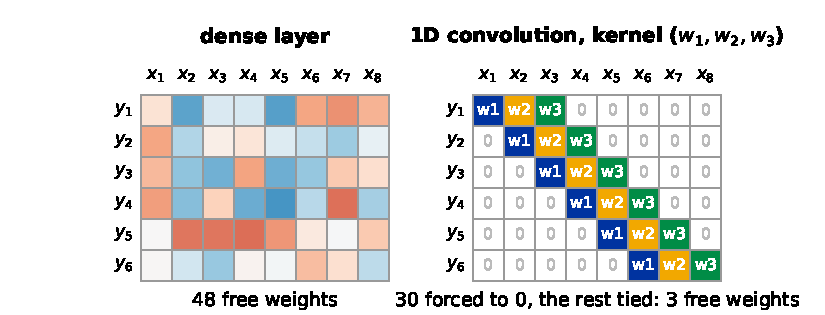
\includegraphics[width=5.0in]{conv_as_matrix.pdf}\end{center}
  \vskip 2pt
  \fcolorbox{armblue}{armblue!8}{\parbox{0.97\linewidth}{\small
    Two constraints: outside the window, weights are \textbf{forced to 0} (locality); every
    row \textbf{reuses the same 3 weights} (sharing). A dense layer \emph{could} learn the
    right-hand matrix; a conv layer can learn \emph{nothing else}.}}
\end{frame}

\begin{frame}{Regularization by architecture}
  \small
  You have met a regularizer that also shrinks the hypothesis space - weight decay ([43]).
  Compare the two:
  \vskip 4pt
  \begin{center}
    \begin{tabular}{l l l}
      & \textbf{weight decay} ([43]) & \textbf{convolution}\\
      \hline
      what it does & pulls every weight \emph{toward} 0 & most weights \emph{exactly} 0,
        the rest tied\\[2pt]
      as a prior & \textbf{soft}: allowed if the data insists & \textbf{infinitely strong}:
        forbidden\\[2pt]
      free weights & 48 (previous slide) & 3\\
    \end{tabular}
  \end{center}
  \vskip 4pt
  Fewer free weights means \textbf{lower variance}: less data is needed to pin them down. The
  price is \textbf{bias} - but only where the assumption is false.
  \vskip 4pt
  \fcolorbox{armblue}{armblue!8}{\parbox{0.97\linewidth}{\small
    \textbf{Predict:} shuffle every image's pixels with one fixed permutation. The MLP does not
    notice (Section 1); for the CNN, "neighbors are related" is now simply false. The strongest
    regularizer is not a penalty - it is the \textbf{right inductive bias}. Trees still win on
    tabular data (ch4, [40]) for the same reason.}}
  \vskip 2pt
  {\scriptsize\color{gray} "Infinitely strong prior": Goodfellow, Bengio \& Courville,
  \emph{Deep Learning} (2016), Sec. 9.4.}
\end{frame}

% (translation-invariance frame removed per instructor request, 2026-07-13)

% ================================================================
\section{The components of a conv layer}

\begin{frame}[plain]
  \vfill
  \begin{center}
    {\Large\color{popblue}\textbf{The components of a conv layer}}\\[0.9em]
    \begin{minipage}{0.82\textwidth}\centering\small
      Four knobs turn the sliding dot product into a real layer: channels, padding, stride,
      pooling.
    \end{minipage}
  \end{center}
  \vfill
\end{frame}

% 2026-10-01 rewrite (instructor: "explain channels better"): the old frame mixed RGB talk with
% a 2-channel example and a tiny TikZ sketch. Now two frames, both figures from
% py_src/multichannel_conv.py (numbers asserted there): one filter across all three channels,
% then a whole layer's shapes (3x32x32 -> 16 filters -> 16x32x32, 448 params).
\begin{frame}{Channels: one filter sees all of them}
  \small
  Color returns: an RGB input is \textbf{three stacked grids}. So a filter is a stack too -
  one $k\times k$ \textbf{slice per input channel}. At each position: multiply each slice with
  its own channel, \textbf{add all three} dot products, add the bias.
  \vskip 4pt
  \begin{center}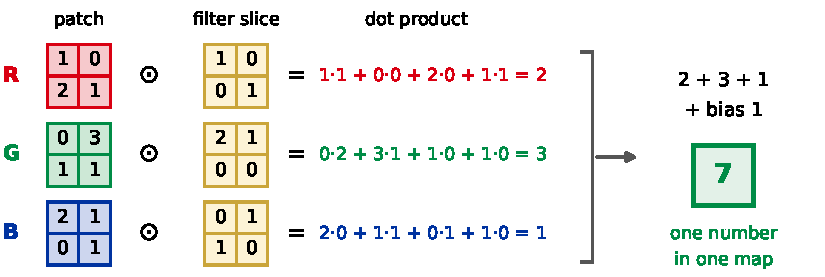
\includegraphics[width=5.5in]{multichannel_conv.pdf}\end{center}
  \vskip 2pt
  \fcolorbox{armred}{armred!8}{\parbox{0.97\linewidth}{\small
    One filter gives \textbf{one number per position}, so \textbf{one feature map} - however
    many channels go in. $3$ channels \emph{in} does not mean $3$ maps \emph{out}. This filter
    has $2\cdot2\cdot3 = 12$ weights $+ 1$ bias.}}
\end{frame}

\begin{frame}{Many filters, many maps}
  \small
  One filter, one map. A real layer learns \textbf{many filters at once} - each its own
  detector - and stacks their maps:
  \vskip 4pt
  \begin{center}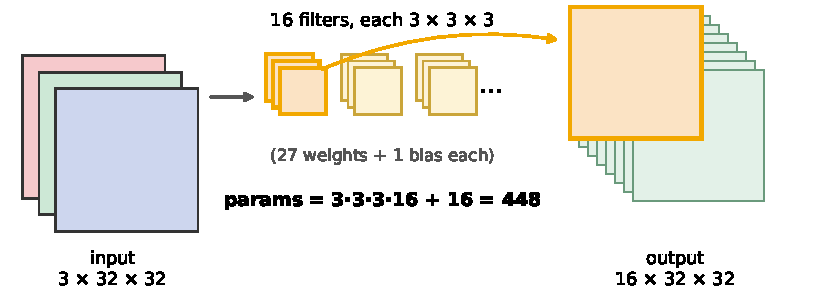
\includegraphics[width=5.5in]{conv_layer_shapes.pdf}\end{center}
  \vskip 2pt
  \fcolorbox{armblue}{armblue!8}{\parbox{0.97\linewidth}{\small
    In general: input $C_{\text{in}} \times H \times W$, $C_{\text{out}}$ filters of size
    $C_{\text{in}} \times k \times k$, output $C_{\text{out}} \times H' \times W'$. The
    \textbf{output depth is the number of filters} - and it becomes the next layer's input
    depth.}}
\end{frame}

\begin{frame}{A whole CNN, end to end}
  Stack such layers and the maps get \textbf{smaller} (pooling) while the stacks get
  \textbf{deeper} (more filters):
  \vskip 2pt
  \begin{center}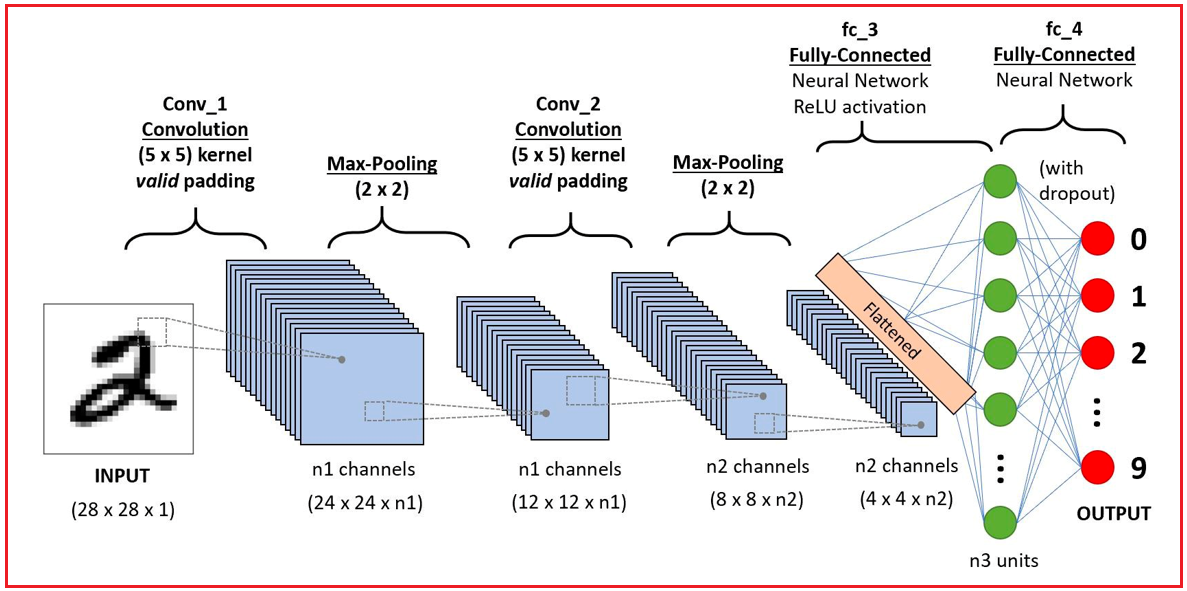
\includegraphics[width=0.72\linewidth]{multi_kernel.png}\end{center}
  \vskip 1pt
  \begin{center}\small
    Conv\_1 learns $n_1$ filters, Conv\_2 learns $n_2$ - then a dense head reads the last stack.
    \\[3pt]
    \href{https://poloclub.github.io/cnn-explainer/}{\beamergotobutton{click through a real
    CNN, layer by layer: CNN Explainer}}
  \end{center}
\end{frame}

\begin{frame}{The conv-layer parameter formula}
  \begin{center}
    \fcolorbox{popblue}{popblue!6}{\parbox{0.8\linewidth}{\centering\large
      $\text{params} = k \cdot k \cdot C_{\text{in}} \cdot C_{\text{out}} + C_{\text{out}}$
      \\[2pt]
      {\footnotesize (one $k\times k$ filter per output channel, spanning the full input
      depth, plus one bias each)}}}
  \end{center}
  \vskip 10pt
  Two cases by hand:
  \begin{itemize}
    \item $3\times3$ conv, RGB $\to 16$ maps: $\;3\cdot3\cdot3\cdot16 + 16 = \textbf{448}$.
    \item the Section-3 $5\times5$ filter on RGB: $\;5\cdot5\cdot3\cdot1 + 1 = \textbf{76}$.
  \end{itemize}
  \vskip 8pt
  \fcolorbox{paramgreen}{paramgreen!8}{\parbox{0.97\linewidth}{\small
      This formula and the output-size formula (next) are the \textbf{two tools} for reading
      any architecture - we use them all through [49] and the homework.}}
\end{frame}

\begin{frame}{Padding: valid vs same}
  \begin{columns}[T]
    \column{0.34\textwidth}
    Without padding, every conv \emph{shrinks} the map - so depth is capped: eventually
    there is nothing left to convolve.
    \vskip 6pt
    Pad the border with zeros ("same" padding) and the output keeps the input's size. Depth
    becomes free.
    \vskip 6pt
    \fcolorbox{armblue}{armblue!8}{\parbox{0.95\linewidth}{\small
      "valid" $=$ no padding (shrinks). "same" $=$ pad to preserve size.}}
    \vskip 4pt
    \href{https://github.com/vdumoulin/conv_arithmetic}{\beamergotobutton{every padding and
    stride case, animated}}
    \column{0.66\textwidth}
    \begin{center}
      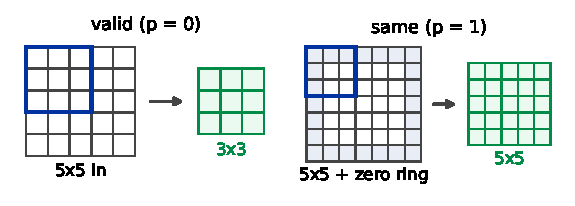
\includegraphics[width=\linewidth]{conv_arithmetic.pdf}
    \end{center}
  \end{columns}
\end{frame}

\begin{frame}{What stride controls}
  \textbf{Stride} $s$ is how far the window jumps between stops. Bigger stride $=$ fewer
  stops $=$ smaller output (and cheaper).
  \vskip 4pt
  \begin{center}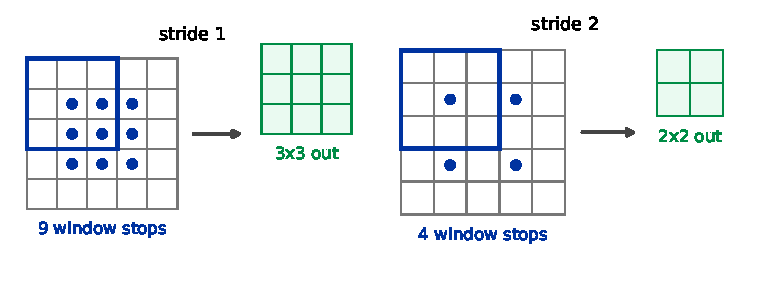
\includegraphics[width=0.92\linewidth]{stride_demo.pdf}\end{center}
\end{frame}

\begin{frame}{Stride and the output-size formula}
  \textbf{Stride} $s$ is how far the window jumps each step. Larger stride $=$ fewer stops
  $=$ smaller output.
  \begin{center}
    \fcolorbox{popblue}{popblue!6}{\parbox{0.6\linewidth}{\centering\large
      $o = \left\lfloor \dfrac{i - k + 2p}{s} \right\rfloor + 1$}}
  \end{center}
  \vskip 6pt
  The classic exam question, three cases:
  \begin{itemize}
    \item $i{=}28,\ k{=}3,\ p{=}1,\ s{=}1:\ \lfloor(28-3+2)/1\rfloor+1 = \textbf{28}$ (same).
    \item $i{=}28,\ k{=}5,\ p{=}0,\ s{=}1:\ \lfloor(28-5)/1\rfloor+1 = \textbf{24}$.
    \item $i{=}32,\ k{=}3,\ p{=}0,\ s{=}2:\ \lfloor(32-3)/2\rfloor+1 = \textbf{15}$.
  \end{itemize}
\end{frame}

\begin{frame}{Pooling}
  Pooling downsamples each map with a small window and \textbf{no weights}. $2\times2$
  windows, stride $2$:
  \vskip 2pt
  \begin{center}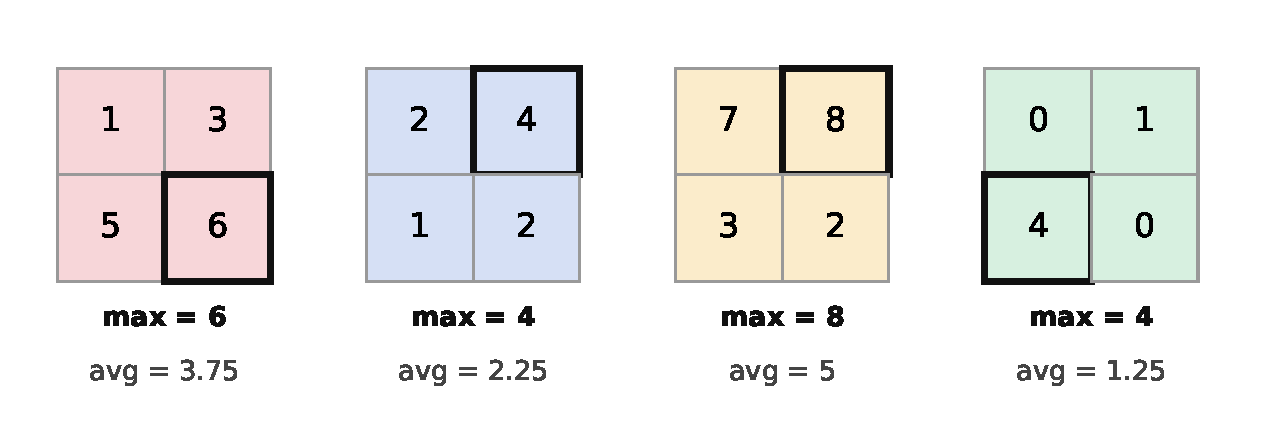
\includegraphics[width=0.90\linewidth]{pooling_demo.pdf}\end{center}
  \vskip 2pt
  \fcolorbox{armblue}{armblue!8}{\parbox{0.97\linewidth}{\small
      \textbf{Max} keeps the strongest response in each window; \textbf{average} smooths.
      Pooling downsamples, cheapens later layers, and buys a little translation invariance.}}
\end{frame}

% ================================================================
\section{Variations on the kernel}

\begin{frame}[plain]
  \vfill
  \begin{center}
    {\Large\color{popblue}\textbf{Variations on the kernel}}\\[0.9em]
    \begin{minipage}{0.82\textwidth}\centering\small
      Same sliding window, three twists: a nonlinear cousin, a kernel with gaps, and a
      kernel that grows the image instead of shrinking it.
    \end{minipage}
  \end{center}
  \vfill
\end{frame}

% 2026-10-01 expansion (instructor: "only results with some titles - explain how it is done"):
% each variation now gets a by-hand frame first (morphology_by_hand, dilated_1d, transposed_steps;
% numbers asserted in their scripts), then the 2D picture, redrawn at slide size.
\begin{frame}{Dilation and erosion, by hand}
  \small
  Not every window operation is a weighted sum. On a \textbf{binary mask} (1 = shape, 0 =
  background), slide a $3\times3$ window and take its \textbf{max} or its \textbf{min}:
  \vskip 4pt
  \begin{center}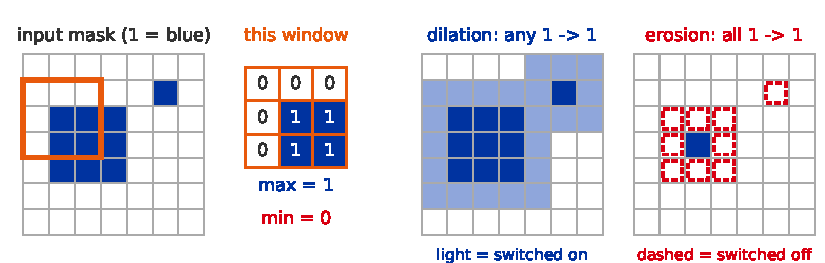
\includegraphics[width=5.5in]{morphology_by_hand.pdf}\end{center}
  \vskip 2pt
  \begin{columns}[T]
    \column{0.49\textwidth}
    \fcolorbox{armblue}{armblue!8}{\parbox{0.95\linewidth}{\small
      \textbf{Dilation} $=$ max: a pixel turns on if \emph{any} pixel in its window is on. The
      shape grows by one pixel all round; nearby blobs merge.}}
    \column{0.49\textwidth}
    \fcolorbox{armred}{armred!8}{\parbox{0.95\linewidth}{\small
      \textbf{Erosion} $=$ min: a pixel stays on only if \emph{every} pixel in its window is
      on. The square shrinks to its center; the stray dot vanishes.}}
  \end{columns}
\end{frame}

\begin{frame}{Dilation and erosion: what they are for}
  \small
  The same two rules on a bigger mask - a square, a square with a hole, a thin line, dots, a plus:
  \vskip 2pt
  \begin{center}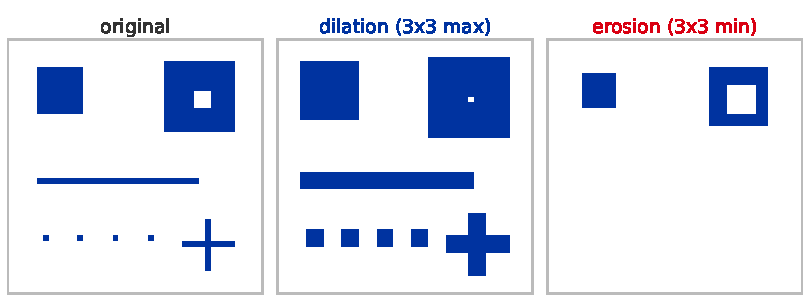
\includegraphics[width=5.4in]{morphology_demo.pdf}\end{center}
  \vskip 2pt
  \fcolorbox{armorange}{armorange!12}{\parbox{0.97\linewidth}{\small
    Dilation fills small holes and thickens lines; erosion deletes dots and thin lines. Chain
    them to \textbf{clean a mask}: erode then dilate (\textbf{opening}) removes specks, dilate
    then erode (\textbf{closing}) fills small holes. Classic pre-CNN tools - and
    \emph{nonlinear}, with \textbf{no weights} to learn.}}
\end{frame}

\begin{frame}{Dilated convolution, by hand}
  \small
  A different idea that shares only the word: \textbf{dilated convolution} keeps the
  weighted sum but spaces the kernel's taps \textbf{$d$ apart}. In 1D, kernel
  $(w_1, w_2, w_3)$:
  \[
    y_i = w_1 x_i + w_2 x_{i+d} + w_3 x_{i+2d}
  \]
  \vskip -4pt
  \begin{center}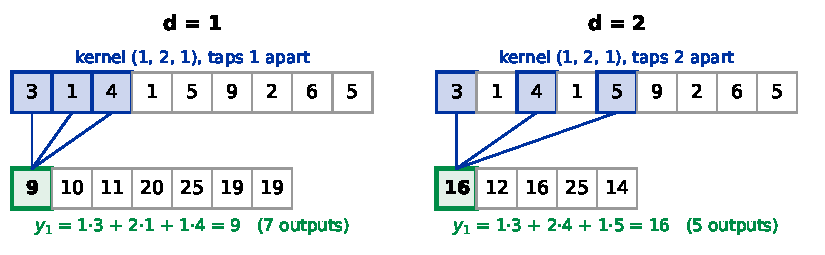
\includegraphics[width=5.5in]{dilated_1d.pdf}\end{center}
  \vskip 2pt
  \fcolorbox{armblue}{armblue!8}{\parbox{0.97\linewidth}{\small
    Same 3 weights, wider reach: a $k$-tap kernel spans $(k-1)d + 1$ inputs - 3 at $d=1$, 5 at
    $d=2$. $d = 1$ \emph{is} the ordinary convolution.}}
\end{frame}

\begin{frame}{Dilated convolution in 2D}
  \small
  A $3\times3$ kernel with dilation $d$ taps cells $d$ apart (green $=$ center tap). The same
  $9$ weights cover a $(2d{+}1)\times(2d{+}1)$ patch - a \textbf{wider receptive field, no
  extra parameters, no pooling}.
  \vskip 2pt
  \begin{center}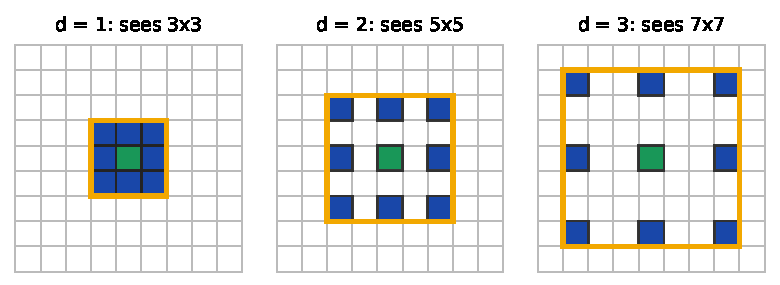
\includegraphics[width=5.2in]{dilated_conv_demo.pdf}\end{center}
  \vskip 2pt
  \fcolorbox{armblue}{armblue!8}{\parbox{0.97\linewidth}{\small
    Stacking layers also widens the view ([49]); dilation does it \emph{within one layer}.
    Back in \textbf{[51]} for segmentation: wide context, every pixel kept.}}
\end{frame}

\begin{frame}{Transposed convolution, step by step}
  \small
  A normal conv \textbf{shrinks} the map; a \textbf{transposed} conv \textbf{grows} it. Each
  input value multiplies the \emph{whole} kernel and \textbf{stamps} it into the output, the
  stride sets how far apart the stamps land, and overlaps \textbf{add}:
  \vskip 2pt
  \begin{center}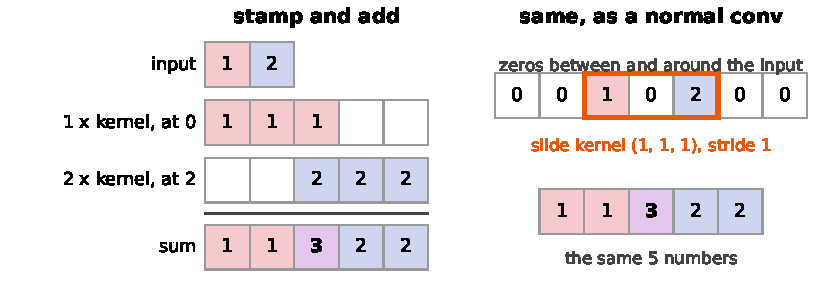
\includegraphics[width=5.3in]{transposed_steps.pdf}\end{center}
  \vskip 2pt
  \fcolorbox{armblue}{armblue!8}{\parbox{0.97\linewidth}{\small
    Length $= s\,(i - 1) + k = 2\cdot1 + 3 = 5$. The right side is why it is a
    \emph{convolution}: spread with zeros, then convolve as usual. The kernel is learned - the
    layer \textbf{learns how to upsample}.}}
\end{frame}

\begin{frame}{Transposed convolution in 2D}
  \begin{columns}[T]
    \column{0.42\textwidth}
    \small
    The same rule on a grid: each of the 4 input cells stamps a $3\times3$ copy of the
    kernel, two cells apart. A $2\times2$ map becomes $5\times5$; the $+$ cells collect two
    stamps.
    \vskip 6pt
    \fcolorbox{armblue}{armblue!8}{\parbox{0.95\linewidth}{\small
      The tool for when the \textbf{output must be an image} - upsampling in \textbf{[51]}'s
      U-Net decoder and in image generators. Uneven overlaps can leave
      \textbf{checkerboard artifacts}.}}
    \column{0.56\textwidth}
    \begin{center}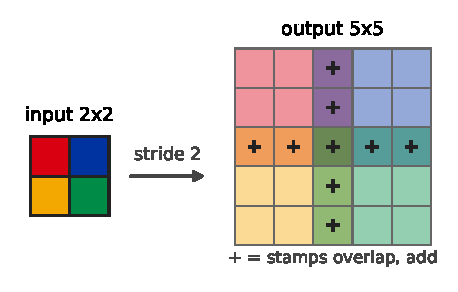
\includegraphics[width=3.05in]{transposed_conv_demo.pdf}\end{center}
  \end{columns}
\end{frame}

% ================================================================
\section{Your first CNN}

\begin{frame}[plain]
  \vfill
  \begin{center}
    {\Large\color{popblue}\textbf{Your first CNN}}\\[0.9em]
    \begin{minipage}{0.82\textwidth}\centering\small
      Stack the blocks, track the tensor, and let autograd do the rest.
    \end{minipage}
  \end{center}
  \vfill
\end{frame}

\begin{frame}{The training loop, in 60 seconds (recall [42])}
  Nothing about training changes for a CNN. The loop from [42], unchanged:
  \vskip 8pt
  \begin{center}
    \begin{tikzpicture}[font=\small, >=Latex, node distance=0.35cm,
      b/.style={draw, rounded corners, minimum height=0.8cm, fill=armblue!10, align=center}]
      \node[b] (f) {forward};
      \node[b, right=of f] (l) {loss};
      \node[b, right=of l] (z) {\texttt{zero\_grad}};
      \node[b, right=of z] (bw) {backward};
      \node[b, right=of bw] (s) {step};
      \draw[->] (f)--(l); \draw[->] (l)--(z); \draw[->] (z)--(bw); \draw[->] (bw)--(s);
      \draw[->] (s) to[bend left=28] (f);
    \end{tikzpicture}
  \end{center}
  \vskip 8pt
  \fcolorbox{paramgreen}{paramgreen!8}{\parbox{0.97\linewidth}{\small
      Forward pass, compute loss, clear old gradients, backprop, update. The only new thing
      today is \emph{which layers} sit inside the forward pass.}}
\end{frame}

% 2026-09-22 addition: closes the "one weight, used everywhere - who updates it?" gap.
% Numbers: x=(1,2,0,3,1), g=(0.5,-1,2): dL/dw = (-1.5, 7, -1), checked by hand and with
% numpy.correlate(x, g, 'valid') in the session scratchpad.
\begin{frame}{Training a shared kernel: the gradients add up}
  \small
  A kernel weight is used at \emph{every} position - so which position updates it?
  \textbf{All of them.} [42]'s chain rule already said so: when a variable feeds several
  outputs, its gradient is the \textbf{sum} over them,
  $\frac{\partial z}{\partial x_i} = \sum_j \frac{\partial z}{\partial y_j}\,
  \frac{\partial y_j}{\partial x_i}$.
  \vskip 4pt
  \begin{columns}[T]
    \column{0.53\textwidth}
    1D, by hand: input $\mathbf{x}=(1,2,0,3,1)$, kernel $(w_1,w_2,w_3)$, so
    $y_j = w_1x_j + w_2x_{j+1} + w_3x_{j+2}$ for $j=1,2,3$. Backprop hands us
    $g_j = \partial L/\partial y_j = (0.5,\,-1,\,2)$. Then
    \[
      \frac{\partial L}{\partial w_1} = \sum_j g_j\,x_j
        = 0.5\cdot1 - 1\cdot2 + 2\cdot0 = -1.5
    \]
    \[
      \frac{\partial L}{\partial w_2} = \sum_j g_j\,x_{j+1}
        = 0.5\cdot2 - 1\cdot0 + 2\cdot3 = 7
    \]
    ($w_2$ met $x_2, x_3, x_4$ - shift by one.) Same way, $\partial L/\partial w_3 = -1$.
    \column{0.44\textwidth}
    \fcolorbox{armblue}{armblue!8}{\parbox{0.95\linewidth}{\small
      The pattern: $\partial L/\partial w_k = \sum_j g_j\,x_{j+k-1}$ - slide $\mathbf{g}$
      along $\mathbf{x}$, take dot products. \textbf{The gradient of a convolution is
      itself a convolution.} In 2D the same, over a 2D window.}}
    \vskip 6pt
    \fcolorbox{paramgreen}{paramgreen!8}{\parbox{0.95\linewidth}{\small
      Sharing helps learning: every kernel weight collects a vote from every position of
      every image in the batch.}}
  \end{columns}
\end{frame}

\begin{frame}{Anatomy of a conv stack}
  \texttt{[conv $\to$ ReLU $\to$ pool] $\times 2$ $\to$ flatten $\to$ dense $\to$ softmax},
  a $28\times28$ input:
  \vskip 4pt
  \begin{center}\footnotesize
    \begin{tabular}{l c r}
      \textbf{Layer} & \textbf{Output shape} & \textbf{Params}\\
      \hline
      input & $1\times28\times28$ & $0$\\
      conv $1{\to}8$, $3\times3$, pad $1$ & $8\times28\times28$ & $80$\\
      ReLU & $8\times28\times28$ & $0$\\
      maxpool $2$ & $8\times14\times14$ & $0$\\
      conv $8{\to}16$, $3\times3$, pad $1$ & $16\times14\times14$ & $1{,}168$\\
      ReLU & $16\times14\times14$ & $0$\\
      maxpool $2$ & $16\times7\times7$ & $0$\\
      flatten & $784$ & $0$\\
      dense $784{\to}10$ & $10$ & $7{,}850$\\
      \hline
      \textbf{total} & & $\mathbf{9{,}098}$\\
    \end{tabular}
  \end{center}
  \vskip 2pt
  \fcolorbox{armorange}{armorange!12}{\parbox{0.97\linewidth}{\small
      Two things to notice: the \textbf{ReLU} matters - without it, stacked convs collapse
      into one big conv ([41\_1]'s linearity lesson); and \textbf{pooling has zero
      parameters}.}}
\end{frame}

\begin{frame}{What the first layer learns}
  \begin{columns}[T]
    \column{0.34\textwidth}
    \small
    Train that CNN on Fashion-MNIST and look at its first-layer kernels (top) and the feature
    maps they produce (bottom): edge and texture detectors \emph{nobody designed}.
    \vskip 6pt
    (Trained on ImageNet, first-layer kernels look like textbook edge detectors - [49].)
    \vskip 6pt
    \fcolorbox{armblue}{armblue!8}{\parbox{0.95\linewidth}{\small
      The first layer is the easy part: it can only see a $3\times3$ patch. What do
      \emph{deeper} layers find?}}
    \column{0.66\textwidth}
    \begin{center}
      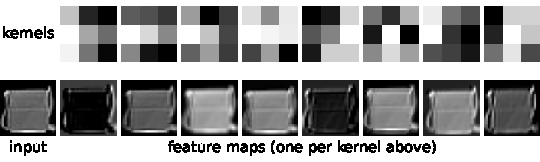
\includegraphics[width=\linewidth]{feature_maps.pdf}
    \end{center}
  \end{columns}
\end{frame}

% 2026-10-01 addition (instructor: "expand on what layers learn"), two frames.
% feature_depth.pdf: torchvision ResNet-18 (ImageNet weights) on the astronaut, two most
% contrasted maps per stage (py_src/feature_hierarchy.py). feature_hierarchy.pdf: Distill's
% hero sprite (Olah, Mordvintsev & Schubert 2017, CC BY 4.0), labels from its source.
\begin{frame}{Feature maps, layer by layer}
  \small
  A pretrained ResNet-18 ([49]) looks at the astronaut. Two feature maps after each of its four
  stages (bright $=$ strong response):
  \vskip 2pt
  \begin{center}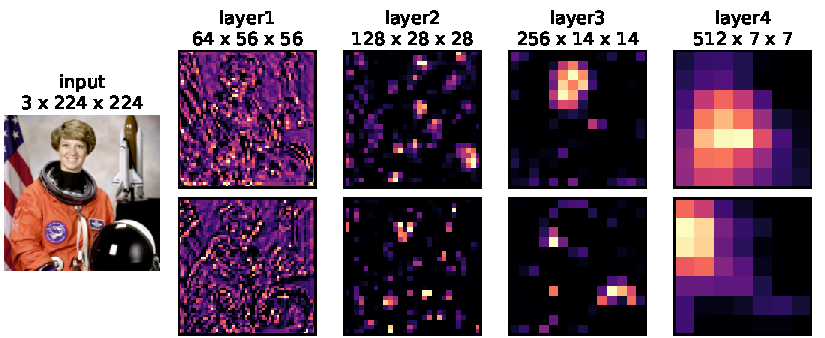
\includegraphics[width=4.9in]{feature_depth.pdf}\end{center}
  \vskip 2pt
  \fcolorbox{armblue}{armblue!8}{\parbox{0.97\linewidth}{\small
    Deeper: a \textbf{coarser} grid ($56 \to 7$), \textbf{more} maps ($64 \to 512$) - less
    \emph{where}, more \emph{what}. Late maps light up on whole regions: the face, the person.}}
\end{frame}

\begin{frame}{What deeper layers look for}
  \small
  \textbf{Feature visualization}: change the \emph{input image} until one channel fires as hard
  as it can - that shows what the channel looks for. Five depths of GoogLeNet (ImageNet):
  \vskip 2pt
  \par{\centering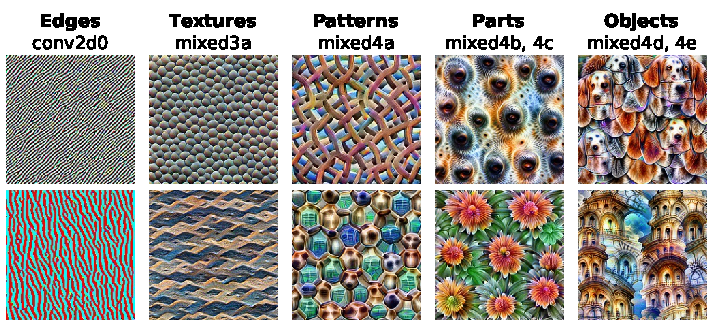
\includegraphics[width=3.9in]{feature_hierarchy.pdf}\par}
  \vskip 2pt
  \fcolorbox{armblue}{armblue!8}{\parbox{0.97\linewidth}{\small
    Edges $\to$ textures $\to$ patterns $\to$ parts $\to$ objects, each built from the one
    below. Nobody told the network these exist: [41\_1]'s XOR lesson at scale.}}
  \vskip 1pt
  {\scriptsize\color{gray} Images: Olah, Mordvintsev \& Schubert, "Feature Visualization",
  Distill (2017), CC BY 4.0.}
  \vskip 1pt
  % Activation Atlas links (instructor request 2026-10-02); all three posts dated 2019-03-06.
  \centering\scriptsize Go deeper:
  \href{https://distill.pub/2017/feature-visualization/}{\beamergotobutton{Feature
  Visualization (Distill)}}
  \href{https://distill.pub/2019/activation-atlas/}{\beamergotobutton{Activation Atlas
  (Distill)}}
  \href{https://openai.com/index/introducing-activation-atlases/}{\beamergotobutton{OpenAI
  blog}}
  \href{https://research.google/blog/exploring-neural-networks-with-activation-atlases/}{\beamergotobutton{Google
  blog}}
\end{frame}

\begin{frame}[fragile]{The canonical snippet}
  The architecture from the anatomy slide, in PyTorch:
\begin{lstlisting}
import torch.nn as nn

net = nn.Sequential(
    nn.Conv2d(1, 8, 3, padding=1),  nn.ReLU(), nn.MaxPool2d(2),
    nn.Conv2d(8, 16, 3, padding=1), nn.ReLU(), nn.MaxPool2d(2),
    nn.Flatten(),
    nn.Linear(16 * 7 * 7, 10),
)
# training loop: unchanged from [42]
# forward -> loss -> zero_grad -> backward -> step
\end{lstlisting}
  \vskip 2pt
  \fcolorbox{paramgreen}{paramgreen!8}{\parbox{0.97\linewidth}{\small
      Autograd differentiates a conv like anything else - [42]'s \texttt{loss.backward()}
      promise (one backward sweep, any graph), kept.}}
\end{frame}

\begin{frame}{Why this is fast}
  A convolution unrolls into a large \textbf{matrix multiply}: every output pixel is a dot
  product, and all of them stack into one big matmul.
  \vskip 8pt
  That is exactly the shape a \textbf{GPU} eats ([42]'s hardware pages) - thousands of
  identical multiply-adds in parallel.
  \vskip 8pt
  \fcolorbox{armblue}{armblue!8}{\parbox{0.97\linewidth}{\small
      Same reason AlexNet's $60$ million parameters trained in under a week on two gaming
      GPUs in 2012 (next lecture): the operation maps perfectly onto parallel hardware.}}
\end{frame}

\begin{frame}{Payoff: CNN vs MLP, same data}
  \begin{columns}[T]
    \column{0.34\textwidth}
    Fashion-MNIST ($28\times28$ grayscale clothing photos, 10 classes), 15k training images,
    15 epochs each: a 784-128-64-10 MLP vs this small CNN.
    \vskip 6pt
    Accuracy is \textbf{about equal}, but the CNN uses \textbf{$12\times$ fewer} weights.
    \vskip 6pt
    \fcolorbox{paramgreen}{paramgreen!8}{\parbox{0.95\linewidth}{\small
      The \emph{architecture}, not raw capacity, did the work. In the \textbf{Gesture
      Snake} practical you train a CNN like this on your own webcam photos - and steer a
      game with it.}}
    \column{0.66\textwidth}
    \begin{center}
      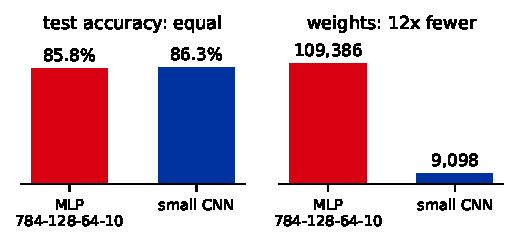
\includegraphics[width=\linewidth]{cnn_vs_mlp.pdf}
    \end{center}
  \end{columns}
\end{frame}

% ================================================================
% 2026-10-02 addition (instructor: "mention CV we don't cover - Canny, template matching,
% Hough and so on, one frame each with nice visuals"; placed before the Recap, not after the
% appendix). Figures: py_src/classical_cv.py; every number quoted is printed in its log.
\section{Classical vision we skip}

\begin{frame}[plain]
  \vfill
  \begin{center}
    {\Large\color{popblue}\textbf{Classical vision we skip}}\\[0.9em]
    \begin{minipage}{0.82\textwidth}\centering\small
      Before CNNs, vision was hand-built from this lecture's kernels. Six classics you will
      still meet in OpenCV - each one is blur, gradients and one clever idea.
    \end{minipage}
  \end{center}
  \vfill
\end{frame}

\begin{frame}{Canny edge detector (1986)}
  \par\vskip 4pt{\centering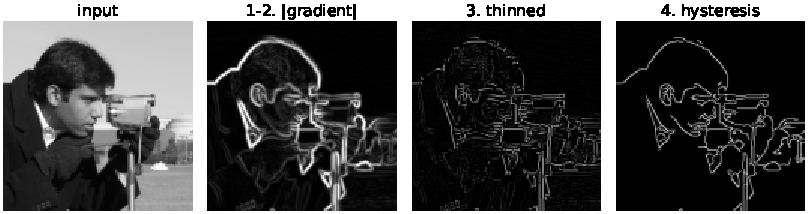
\includegraphics{cv_canny.pdf}\par}
  \vskip 2pt
  \begin{columns}[T]
    \column{0.53\textwidth}
    \footnotesize
    \begin{enumerate}\setlength\itemsep{0pt}
      \item \textbf{Blur} (Gaussian), or noise becomes edges.
      \item \textbf{Sobel} X and Y: gradient strength and direction.
      \item \textbf{Thin}: keep only the maxima along the gradient (1 px wide).
      \item \textbf{Hysteresis}: strong pixels are edges; weak ones only if they touch a
        strong one.
    \end{enumerate}
    \column{0.45\textwidth}
    \footnotesize
    John Canny's detector is still the default, \texttt{cv2.Canny(img, 50, 150)}: document
    scanners, measuring parts on a factory line.
    \vskip 4pt
    \fcolorbox{armorange}{armorange!12}{\parbox{0.95\linewidth}{\footnotesize
      The two thresholds are hand-tuned - per camera, per lighting.}}
  \end{columns}
\end{frame}

\begin{frame}{Template matching}
  \par\vskip 4pt{\centering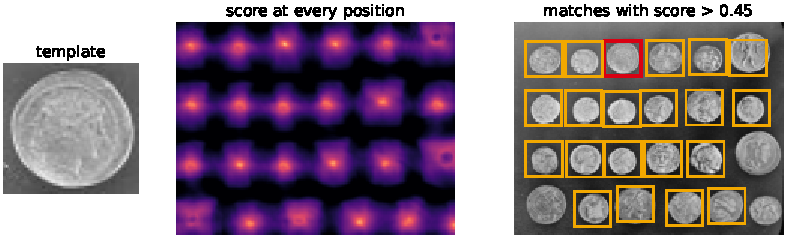
\includegraphics{cv_template.pdf}\par}
  \vskip 2pt
  \begin{columns}[T]
    \column{0.53\textwidth}
    \footnotesize
    Slide the \textbf{template} over the image and score every position by
    \textbf{normalized cross-correlation}: a convolution whose kernel \emph{is} the template,
    brightness divided out. Peaks are matches.
    \vskip 3pt
    \texttt{cv2.matchTemplate}: UI test bots, circuit-board checks - wherever the target
    always looks the same.
    \column{0.45\textwidth}
    \footnotesize
    From one coin it finds 21 of the 24 (score $>0.45$, red $=$ the template itself).
    \vskip 4pt
    \fcolorbox{armorange}{armorange!12}{\parbox{0.95\linewidth}{\footnotesize
      The 3 it misses include the 2 biggest: it has no idea of \textbf{scale} or
      \textbf{rotation}. Change either and the score collapses.}}
  \end{columns}
\end{frame}

\begin{frame}{Hough transform: finding lines by voting}
  \par\vskip 4pt{\centering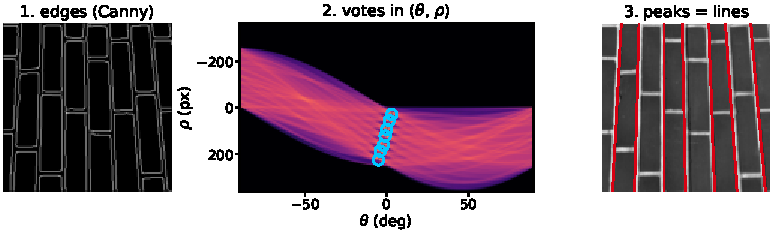
\includegraphics{cv_hough.pdf}\par}
  \vskip 2pt
  \begin{columns}[T]
    \column{0.53\textwidth}
    \footnotesize
    \begin{enumerate}\setlength\itemsep{0pt}
      \item Find edges (Canny).
      \item Every edge pixel \textbf{votes} for every line through it. A line is
        $x\cos\theta+y\sin\theta=\rho$, so one pixel's votes trace a sinusoid in
        $(\theta,\rho)$.
      \item Where many sinusoids cross, many pixels agree on one line: \textbf{peaks are
        lines}.
    \end{enumerate}
    \column{0.45\textwidth}
    \footnotesize
    Paul Hough patented it in 1962 to follow particle tracks in bubble-chamber photos; Duda
    \& Hart (1972) gave it the $(\theta,\rho)$ form. \texttt{cv2.HoughLines}: lane lines,
    document edges. The same voting finds circles (\texttt{cv2.HoughCircles}): coins, pupils,
    wheels.
  \end{columns}
\end{frame}

\begin{frame}{Harris corner detector (1988)}
  \par\vskip 4pt{\centering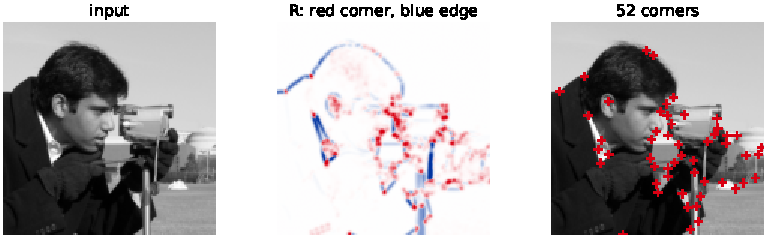
\includegraphics{cv_harris.pdf}\par}
  \vskip 2pt
  \begin{columns}[T]
    \column{0.53\textwidth}
    \footnotesize
    A \textbf{corner} changes in \emph{two} directions. From Sobel gradients $I_x, I_y$,
    averaged over a small window:
    \[
      M=\sum_{\text{window}}\begin{bmatrix}I_x^2 & I_xI_y\\ I_xI_y & I_y^2\end{bmatrix},\qquad
      R=\det M-k\,(\operatorname{tr}M)^2.
    \]
    Two large eigenvalues: corner ($R>0$). One: edge ($R<0$). None: flat.
    \column{0.45\textwidth}
    \footnotesize
    Harris \& Stephens, 1988. Corners are the points you can find \emph{again} in the next
    frame: tracking, video stabilization, AR anchors, panoramas. \texttt{cv2.cornerHarris},
    or \texttt{cv2.goodFeaturesToTrack} (Shi \& Tomasi, 1994).
  \end{columns}
\end{frame}

\begin{frame}{SIFT: features that survive rotation and zoom}
  \par\vskip 4pt{\centering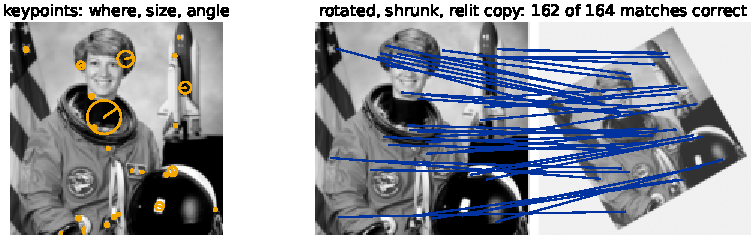
\includegraphics{cv_sift.pdf}\par}
  \vskip 2pt
  \begin{columns}[T]
    \column{0.53\textwidth}
    \footnotesize
    \begin{enumerate}\setlength\itemsep{0pt}
      \item Blur at many scales; \textbf{keypoints} are blobs that stand out.
      \item Each gets its main gradient \textbf{angle}: rotation undone.
      \item Gradient-angle histograms, $4\times4$ cells $\times$ 8 angles: a
        \textbf{128-number fingerprint}.
      \item Match fingerprints by nearest neighbour.
    \end{enumerate}
    \column{0.45\textwidth}
    \footnotesize
    Scale-Invariant Feature Transform (David Lowe, 1999/2004). Panorama stitching, 3D models
    from photos, robot localization. Patented until March 2020 - now free in
    \texttt{cv2.SIFT\_create()}.
  \end{columns}
\end{frame}

\begin{frame}{HOG: histograms of oriented gradients (2005)}
  \par\vskip 4pt{\centering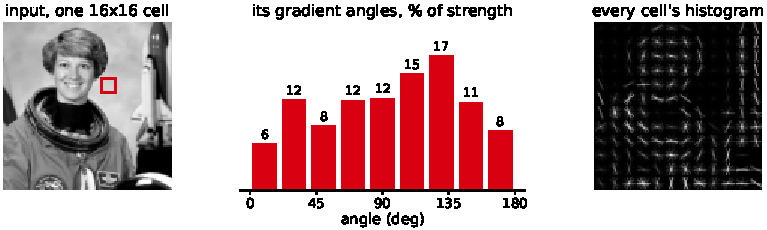
\includegraphics{cv_hog.pdf}\par}
  \vskip 2pt
  \begin{columns}[T]
    \column{0.53\textwidth}
    \footnotesize
    \begin{enumerate}\setlength\itemsep{0pt}
      \item Sobel gradients everywhere.
      \item Cells ($8\times8$ in the paper, $16\times16$ here): each histograms its
        gradient angles into 9 bins, weighted by strength.
      \item Normalize over $2\times2$ blocks (lighting), concatenate, and a linear classifier
        (an SVM) says person / not person.
    \end{enumerate}
    \column{0.45\textwidth}
    \footnotesize
    Dalal \& Triggs, 2005 - the pedestrian detector of the 2000s.
    \vskip 4pt
    \fcolorbox{armblue}{armblue!8}{\parbox{0.95\linewidth}{\footnotesize
      HOG is a \textbf{hand-built CNN layer}: fixed kernels, binning, pooling, a linear
      classifier. This whole section is kernels plus hand-made rules; a CNN learns both.}}
  \end{columns}
\end{frame}

% ================================================================
\section*{Recap}

\begin{frame}{Recap}
  \begin{itemize}
    \item A dense net cannot afford pixels and ignores their structure.
    \item Convolution $=$ a \textbf{local}, \textbf{shared} neuron - a dense layer with most
      weights forced to 0 and the rest tied: an infinitely strong prior.
    \item One filter spans the \emph{full input depth} and outputs \emph{one} feature map;
      $N$ filters $\to N$ maps. Deeper maps: coarser, more of them, more abstract.
    \item Two formulas run everything: $o=\lfloor(i-k+2p)/s\rfloor+1$ and
      $\text{params}=k\,k\,C_{\text{in}}C_{\text{out}}+C_{\text{out}}$.
    \item Pooling has \textbf{zero parameters}; it downsamples and buys a little invariance.
    \item Kernels are \textbf{learned}, not hand-designed - a shared weight's gradient is
      the \textbf{sum} over every position it touched.
  \end{itemize}
  \vskip 6pt
  \fcolorbox{paramgreen}{paramgreen!8}{\parbox{0.97\linewidth}{
      \textbf{Next:} we can build a small CNN. What did 10 years of architecture design buy?
      The ImageNet story - from $26\%$ error to superhuman ([49]).}}
\end{frame}

% ================================================================
% APPENDIX (2026-10-01, instructor request): the Fourier detour, moved out of Section 2.
\appendix
\section*{Appendix: convolution in frequency space}

\begin{frame}[plain]
  \vfill
  \begin{center}
    {\Large\color{popblue}\textbf{Appendix: convolution in frequency space}}\\[0.9em]
    \begin{minipage}{0.82\textwidth}\centering\small
      For the curious: why a kernel is a frequency filter, and why big convolutions are
      computed with the fast Fourier transform. The full math, with proofs, is in the optional
      deck \emph{The Convolution, Mathematically}.
    \end{minipage}
  \end{center}
  \vfill
\end{frame}

\begin{frame}{From Taylor to Fourier}
  \begin{center}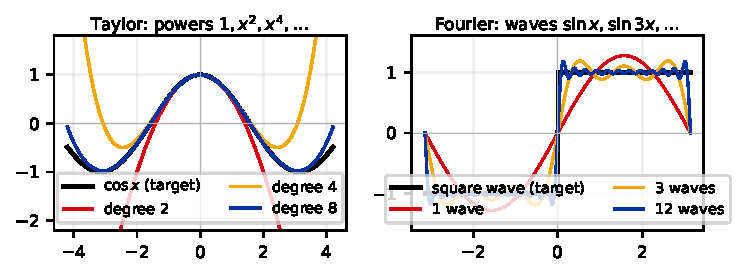
\includegraphics[width=0.92\linewidth]{taylor_vs_fourier.pdf}\end{center}
  \vskip 4pt
  \begin{columns}[T]
    \column{0.60\textwidth}
    You already know \textbf{Taylor}: rebuild a function as a sum of \textbf{powers}
    $1, x, x^2, \ldots$ - a great fit near a point. \textbf{Fourier} is the same move with
    different blocks: a sum of \textbf{waves} $\sin x, \sin 2x, \ldots$ of rising
    \emph{frequency}, and it fits everywhere.
    \column{0.40\textwidth}
    \fcolorbox{armblue}{armblue!8}{\parbox{0.95\linewidth}{\small
      Both break a function into simple pieces. Taylor's are powers; Fourier's are labelled by
      \textbf{frequency}.}}
  \end{columns}
\end{frame}

\begin{frame}{A signal is a bundle of frequencies}
  \begin{center}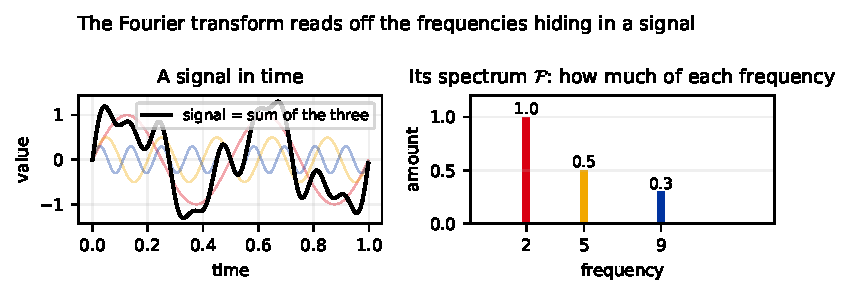
\includegraphics[width=0.97\linewidth]{spectrum_1d.pdf}\end{center}
  \vskip 4pt
  \begin{columns}[T]
    \column{0.60\textwidth}
    Add three sine waves and you get one wiggly signal. The \textbf{Fourier transform}
    $\mathcal{F}$ runs it backwards: it reads off \emph{how much of each frequency} sits inside
    - three tones in, three clean spikes out. That is the signal's \textbf{spectrum}.
    \column{0.40\textwidth}
    \fcolorbox{armblue}{armblue!8}{\parbox{0.95\linewidth}{\small
      Same information, two views: the wave in time, or its recipe in frequency.}}
  \end{columns}
\end{frame}

\begin{frame}{Convolution lives in frequency too}
  The payoff is one clean fact - the \textbf{convolution theorem}:
  \vskip 6pt
  \[
    \mathcal{F}\{f \ast g\} \;=\; \mathcal{F}\{f\}\,\cdot\,\mathcal{F}\{g\}
  \]
  \vskip 4pt
  \textbf{Convolving in space $=$ multiplying in frequency.} The messy slide-and-sum turns into
  a plain pointwise product once you switch to the frequency view.
  \vskip 6pt
  So the fast way to convolve a large image with a large kernel is to take the \textbf{fast
  Fourier transform} (FFT) of both, multiply, and transform back:
  \[
    f \ast g \;=\; \mathcal{F}^{-1}\!\big\{\,\mathcal{F}\{f\}\cdot\mathcal{F}\{g\}\,\big\}.
  \]
  \vskip 4pt
  \fcolorbox{armblue}{armblue!8}{\parbox{0.97\linewidth}{\small
    A kernel is a \textbf{frequency filter}: it scales each frequency of the image up or down.}}
\end{frame}

\begin{frame}{Blur and edges are frequency filters}
  \begin{columns}[T]
    \column{0.48\textwidth}
    Send the image to frequency space - its \textbf{spectrum} (top right: bright centre $=$
    low frequencies $=$ smooth areas; outer $=$ high $=$ fine detail and edges).
    \vskip 6pt
    \textbf{Keep the low} frequencies and you get a \textbf{blur}. \textbf{Keep the high} ones
    and you are left with \textbf{edges}.
    \vskip 6pt
    \fcolorbox{armblue}{armblue!8}{\parbox{0.95\linewidth}{\small
      You met both as kernels in Section 2: the \textbf{box blur} is a low-pass filter, and \textbf{Sobel} is a high-pass one.}}
    \column{0.52\textwidth}
    \begin{center}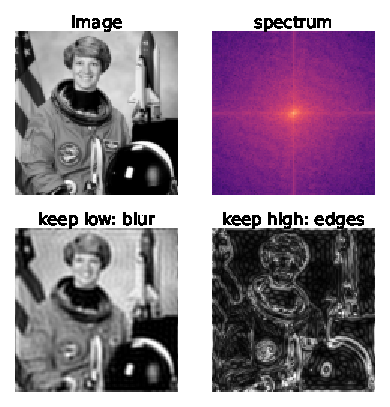
\includegraphics[height=2.6in]{fourier_view.pdf}\end{center}
  \end{columns}
\end{frame}

\end{document}

% ================================================================
% Provenance:
%   Deck: L16 CNN Foundations (12_cnn). Built 2026-07-13 from
%   48_cnn_foundations_OUTLINE.md (approved) + CNN_CHAPTER_PLAN.md.
%   (Chapter wrap-up 2026-10-17: the OUTLINE / QUESTIONS / NN_DECISIONS / HW1b_photoshop_PLAN
%   files named in these notes were deleted; `git show 1a62099:ml/12_cnn/<file>` recovers them.)
%
%   Sources consulted (REDERIVE, read-only): LMU I2DL cnn1/{conv2d,
%   properties-of-convolution, components, pooling, architecture}.tex; 1D-first idea from
%   cnn2/convolution-types. Credit line on title frame per instructor decision (CC BY 4.0).
%
%   Figures (py_src -> fig, ma venv): image_numbers.pdf, pixel_shuffle.pdf (pixel_shuffle.py);
%   kernel_zoo.pdf (kernel_zoo.py, naive NumPy conv = HW1 Part A loop); param_explosion.pdf;
%   conv_arithmetic.pdf; feature_maps.pdf + cnn_vs_mlp.pdf (feature_maps.py, cnn_vs_mlp.py -
%   chapter SmallCNN, 9098 params, 15k Fashion-MNIST subsample, 15 epochs, seed 509).
%   Borrowed montage images (COPY-IMG whitelist, fig/borrowed/): tesla_autopilot.jpg,
%   coronatrack.jpeg, cityscapes_visual.png, colorization.png.
%
%   Key decisions:
%   - cnn_vs_mlp reframed as accuracy(tie)+params(12x) bars, NOT accuracy-vs-epoch: on
%     Fashion-MNIST the two nets tie (~86%), so the curve read as "MLP wins" (false to the
%     lesson). The honest, clear payoff is parameter efficiency. Config bumped from the
%     plan's 8k/5ep (where the MLP won) to 15k/15ep + full 10k test (CNN edges ahead).
%   - No photo credit line (instructor instruction 2026-07-13: assets I'm told to use are
%     cleared; do not add licensing/credit notes for them).
%   - 7 kernels incl. Gaussian (reviewer B1); training-loop recap frame included (B2).
%
%   v2 revision (2026-07-13, instructor requests): expanded the image-fundamentals front
%   half and added visual/animated aids. New figures (py_src -> fig, ma venv):
%   eye_cones.pdf (trichromacy), rgb_channels.pdf + kernel_zoo.pdf + sobel_build.pdf (now on
%   skimage's public-domain 'astronaut' test image - the ethical Lena replacement, per the
%   "better demo image / Lera" request), image_as_function.pdf (synthetic image + horizontal
%   intensity profiles), edge_1d.pdf (edge = derivative = difference of neighbours),
%   conv_anim_0..8.pdf (9-frame flip-book convolution animation, shown via \only<n>),
%   stride_demo.pdf, pooling_demo.pdf. New frames: eye/RGB, image-as-function, "Where CNNs
%   came from" (LeCun/MNIST/LeNet), the animation, a 3-frame edges-as-derivatives arc
%   (replacing the single Sobel-dissected frame), "What stride controls", visual pooling.
%   REMOVED: the translation-invariance myth-buster frame (instructor request); recap bullet
%   updated to match. Pomegranate stays only as the cold-open running example.
%
%   v3 revision (2026-07-13, instructor requests): 1D case expanded - new frames
%   "moving average is a convolution" (moving_average.pdf) and "convolution lives in
%   probability too" (dice_conv.pdf: two-dice sum = convolution of uniforms). conv_anim
%   redesigned: a Gaussian-blur kernel computing a WEIGHTED AVERAGE (/16) on a value-shaded
%   grayscale patch, fixed geometry (no click-jitter). New "A layer has many kernels" frame
%   embedding multi_kernel.png (LeNet pipeline, downloaded per instructor - shows the map
%   stacks). Fixed the slide-18 formula/figure overlap on the edge-derivative frame.
%   pooling_demo redesigned to a 1x4 row of the four windows (max/avg each). Demo image for
%   operations is skimage 'astronaut' (public domain).
%
%   v4 revision (2026-07-17, instructor request): added a 4-frame Fourier aside after the
%   dice slide - REVERSES the CNN_CHAPTER_PLAN.md decision to skip conv-theorem/Fourier as
%   "too deep". Kept the statement + intuition, dropped the LMU Fubini proof (house style).
%   Framed for students who know Taylor but not Fourier. New frames: "from Taylor to Fourier",
%   "a signal is a bundle of frequencies", "convolution lives in frequency too" (the theorem
%   F{f*g}=F{f}F{g}, conv-in-space = multiply-in-frequency, FFT-is-fast), "blur and edges are
%   frequency filters" (primes the kernel zoo: box blur = low-pass, Sobel = high-pass).
%   New figures (py_src -> fig, ma venv): taylor_vs_fourier.pdf (cos from powers | square wave
%   from waves), spectrum_1d.pdf (3 tones -> 3 spectral spikes), fourier_view.pdf (astronaut +
%   2D FFT + low-pass=blur / high-pass=edges, same 'astronaut' image as kernel_zoo). Also
%   dropped "No Fourier transforms required." from the cross-correlation footnote (now stale).
%   Source: LMU I2DL cnn1/slides-cnn-math.tex (statement only, proof intentionally omitted).
%
%   v5 revision (2026-07-21, instructor request): new section "Variations on the kernel"
%   after the components section (before "Your first CNN") - dilation/erosion, dilated conv,
%   transposed conv, all "quite visual" per request. New figures (py_src -> fig, ma venv):
%   morphology_demo.pdf (pure-numpy 3x3 max/min on a synthetic binary shape: original |
%   dilation | erosion; nonlinear, flagged as NOT a weighted-sum conv), dilated_conv_demo.pdf
%   (one 3x3 kernel at d=1,2,3 -> receptive field 3/5/7, same 9 weights), transposed_conv_demo.pdf
%   (2x2 -> 5x5 stamp-and-add upsampling). Dilated + transposed are also covered in L19
%   (segmentation); L16's versions are the visual intuition, cross-referenced to L19. Prompted
%   by the 3Blue1Brown convolution video (see _reference_3b1b_convolution/). Same date: the
%   Sobel-build frame now names its (column)x(row) factorization "spatially separable"
%   (naming-gap fix from the conv-type coverage check).
%
%   v6 revision (2026-08-02, instructor request): new frame "Three numbers, but which three?"
%   in Section 1, between the RGB-channels frame and the grid-of-numbers frame - HSV as a
%   re-coordinatisation of the same pixel (H = angle/which color, S = radius/how pure,
%   V = height/how bright). Added so HW1b ("Photoshop from scratch", see
%   HW1b_photoshop_PLAN.md) has a slide to call back to; its Part 3 does hue rotation,
%   desaturation and selective-color on top of this. New figure (py_src -> fig, ma venv):
%   hsv_space.pdf - top row astronaut + H/S/V channels (same image as rgb_channels.pdf),
%   bottom row the payoff (RGB subtract vs RGB multiply vs HSV V-scale vs H rotation).
%   Slide numbers are MEASURED by the script, not asserted: subtracting 110 shifts hue a mean
%   20.4 deg over the 48.3% of pixels with S>0.2 and crushes 30.9% to pure black. The script
%   also asserts that scaling V is exactly a uniform RGB multiply (max gap 2.5e-16) - so the
%   slide's claim is about RGB's AMBIGUITY, not about RGB being unable to darken cleanly.
%   One adjacent line edited by necessity: the next frame's "We just saw color as three
%   stacked grids" -> "RGB or HSV, color is three stacked grids".
%
%   v7 revision (2026-09-22, pre-delivery pedagogy pass, instructor away - autonomous):
%   - Retired-deck callbacks repointed to what was actually delivered: L14/L15 no longer
%     exist; every callback was checked against the [40]-[45] .tex AND the LMU page text
%     they embed (pdftotext). Cold open now quotes the ch11 homework MLP (784-256-128-10 =
%     235,146 weights, counted from nn_practical_solution.ipynb) instead of L14's 109,386.
%     L02 -> [02], L01g -> [26], L14 neuron/XOR/linearity -> [41_1], L15 weight decay ->
%     [43], L15 loop -> [42] + homework, why-GPUs -> [42] (LMU hardware pages), tabular
%     caveat -> [40] (LMU 01_introduction).
%   - Colour section: the three cones/RGB/HSV frames folded into ONE recap frame
%     ("Color, recalled from [33]") - deck 33 taught all of it on 2026-08-20. Resolves the
%     DEFERRED_TODO "trim L16's colour section" item. Figures and py_src kept on disk.
%   - NEW "Nature had the same two wishes" (Hubel & Wiesel simple/complex cells -> conv /
%     pooling, Nobel 1981) and a rewritten "Where CNNs came from" timeline (Fukushima's
%     neocognitron 1980 -> LeCun 1989 -> LeNet-5 + MNIST 1998). Web-verified 2026-09-22.
%     "CNNs in the wild" moved after the timeline.
%   - "Two wishes" now names translation equivariance (L19's inductive-bias ledger used the
%     term and nothing defined it since the myth-buster frame was removed 2026-07-13).
%   - NEW "Training a shared kernel: the gradients add up" (1D by-hand example, dL/dw =
%     (-1.5, 7, -1), verified with numpy.correlate and finite differences).
%   - Fixes: dilated-conv frame said "L17 grew the receptive field" inside L16 (a lecture
%     that has not happened yet); canonical snippet said "Section-5 architecture" (the
%     anatomy table is in Section 6 since v5); payoff frame claimed "the same subsample and
%     epochs as the ch5 practical" (false: figure is 15k/15 epochs vs the homework's 10k) and
%     pointed to L17 for a CNN-vs-MLP chasm L17 never shows; "trains overnight" for a 60M
%     CNN replaced by AlexNet's measured "under a week on two GPUs".
%
%   2026-10-01 round 2 (instructor's 13-point list for L16):
%   - Cold open: the ch11-homework MLP is gone (no such homework any more); the 150M-weight
%     dense layer is now compared with GPT-2 small (~124M parameters). The other three "ch11
%     homework" mentions (training loop, snippet comment, payoff data) now point to [42] or say
%     what Fashion-MNIST is.
%   - "Where CNNs came from": 1989 and 1998 read as two attempts; now one ten-year Bell Labs
%     project (1989 ZIP codes = LeNet-1's prototype, refined to LeNet-5, check reading, 1998
%     write-up + MNIST). Web-checked 2026-10-01.
%   - NEW full-bleed "Must watch" frame after the Outline: 3Blue1Brown, "But what is a
%     convolution?" (KuXjwB4LzSA), still = fig/borrowed/3b1b_mario_kernel.jpg.
%   - Color frame: one line on the astronaut (Eileen Collins, NASA, public domain) replacing
%     "Lena" (1972 Playboy scan; IEEE stopped accepting it in 2024). Web-checked 2026-10-01.
%   - The 4-frame Fourier aside moved to an \appendix after the Recap (pointer on the dice frame).
%   - "2D convolution, by hand" now DEFINES feature map (first use of the term).
%   - conv_anim redrawn at slide size with an orange window (the blue one vanished on dark cells).
%   - "Regularization by architecture" -> two frames: conv as a constrained dense matrix
%     (conv_as_matrix.py, 48 free weights vs 3) and weight decay (soft prior) vs convolution
%     ("infinitely strong prior", Goodfellow et al. 2016, Sec. 9.4) + pixel-shuffle predict.
%   - "Channels, done properly" -> "Channels: one filter sees all of them" (multichannel_conv,
%     R+G+B+bias = 7) and "Many filters, many maps" (conv_layer_shapes, 448 params); the LeNet
%     image frame is now "A whole CNN, end to end".
%   - Variations: each gets a by-hand frame before its 2D picture - morphology_by_hand (window
%     max/min, opening/closing on the results frame), dilated_1d ((k-1)d+1 reach), and
%     transposed_steps (stamp-and-add = zero-insert + ordinary conv, o = s(i-1)+k). The three
%     2D figures were redrawn at slide size. A note separates morphological "dilation" from
%     "dilated convolution".
%   - "What the layers learn" -> three frames: first layer (Fashion-MNIST, existing figure),
%     NEW "Feature maps, layer by layer" (ResNet-18 on the astronaut, feature_hierarchy.py) and
%     NEW "What deeper layers look for" (Distill feature-visualization strip, CC BY 4.0).
%   - Every figure redrawn or added this round is drawn at its slide size and embedded at its
%     native width, so its labels are 7.5-12 pt on the slide.
%
%   2026-10-01 pass (instructor request "improve slides"): payoff box no longer promises
%   "CIFAR-10, HW2 ... the gap becomes a chasm" (HW2 never built, the chasm never measured) -
%   it points to the Gesture Snake practical instead (DECISIONS #58). FFT spelled out on the
%   convolution-theorem frame; "GAN generators" (a forward acronym) -> "image generators";
%   the channels frame's patch/filter matrices now sit in a 2x2 tabular (the inline version
%   wrapped "G=" onto its own line). Figure text is still drawn 2-4x too wide for its slot
%   (2.4-5pt on the slide); a redraw was offered and declined for now.
%
%   2026-10-01 round 3 (instructor: "sure redraw"): every remaining figure redrawn at its slot
%   size; non_essential/detect_small_figure_text.py now reports 0 pages under 5.5 pt (28 pages
%   on the committed PDF). cnn_vs_mlp.py / feature_maps.py retrained once (2 threads, ~4 + ~2
%   min), results cached in ml/12_cnn/results/ and redrawn with --plot-only: MLP 85.8% vs CNN
%   86.3% (payoff wording "about equal, 12x fewer" still holds; 109,386 / 9,098 = 12.0).
%   feature_maps gained "input" / "feature maps" labels; fourier_view went 1x4 -> 2x2 (panels
%   were ~0.5 in wide) with the high-pass panel's contrast stretched. Interactive links added:
%   setosa.io image kernels (kernel zoo), CNN Explainer (whole CNN), vdumoulin/conv_arithmetic
%   (padding); the appendix transition names the optional deck "The Convolution, Mathematically".
%
%   2026-10-02 (instructor): (1) three "Kernel zoo, up close" frames (kernel_gallery.py): each
%   kernel drawn as a grid of its real values, red > 0 / blue < 0, above its output; blur and
%   edges right after the zoo frame, Gabor after Sobel (Jones & Palmer 1987, J Neurophysiol
%   58(6), checked). The first one says kernel = filter = convolution matrix (GIMP) = mask.
%   (2) New section "Classical vision we skip" BEFORE the Recap (instructor: "at the end" means
%   before the appendix): Canny, template matching, Hough, Harris, SIFT, HOG, one frame each
%   (classical_cv.py). Numbers on the slides come from its log: 21 of 24 coins matched, 0 false
%   (the 3 misses include the 2 biggest coins); SIFT 162 of 164 matches correct under a known
%   30-degree / 0.7x warp. SIFT patent expiry (March 2020, OpenCV 4.4) checked. (3) "Go deeper"
%   links on "What deeper layers look for": Feature Visualization, Activation Atlas (Distill),
%   OpenAI and Google blog posts (all three atlas posts dated 2019-03-06, URLs checked).
%
%   Forward pointer: L17 CNN Architectures - ImageNet story LeNet -> AlexNet -> VGG -> ResNet;
%   ResNet residual = "boosting in depth" (ch4 callback). torchvision needed for L17
%   pretrained_filters.py (install into ma before starting L17).
%
%   2026-10-15: renumbered to the playlist after delivery (instructor: no practical between
%   [48] and transfer learning): [50] -> [49], [51] -> [50], [52] -> [51], the practical
%   [53] -> [52]; deck files renamed to match. Slide text uses the new labels; labels written in
%   this block before this date keep the old ones.
